%!TEX root = ../larxxia.tex

\section{Linearly independent vectors may form a basis}
\label{sec:lisb}

\secttoc
\begin{comment}
\pooliv{p.92--7,198--208} \holti{\S2.3}
\end{comment}

\index{linearly dependent|(}
\index{linearly independent|(}
\index{linear dependence|(}
\index{linear independence|(}


In \cref{ch:eesm} on symmetric matrices, the \idx{eigenvector}s from \idx{distinct eigenvalues} are proved to be always \idx{orthogonal}---because of matrix symmetry.  
For general matrices, the eigenvectors are not orthogonal---as introduced at the start of this \cref{ch:gee}.  
But the orthogonal property is extremely useful.
Question: is there some analogue of orthogonality that is similarly useful for general matrices?
Answer: yes. 
We now extend ``orthogonal'' to the more general concept of \text{``linearly independent''.}

One reason that \idx{orthogonal vectors} are useful is that they can form an \idx{orthonormal basis} and hence act as the unit vectors of an orthogonal coordinate systems.
Analogously, the concept of linearly independent vectors is closely connected to \idx{coordinate system}s that are not orthogonal.



\paragraph{Subspace \idx{coordinate system}s} 
In any given mathematical problem, an application wants two things from a \idx{general solution}: 
\begin{itemize}
\item firstly, the general solution must encompass every possibility (the solution must span the possibilities); and 
\item secondly, each possible solution should have a unique algebraic form in the general solution.
\end{itemize}
For an example of the need for a unique algebraic form, let's suppose we wanted to find solutions to the \idx{differential equation} \(d^2y/dt^2-y=0\)\,. 
You might find \(y=3e^x+2e^{-x}\), whereas I find \(y=5\cosh x+\sinh x\), and a friend finds \(y=e^x+4\cosh x\).
It appears from these disparate algebraic forms that we all disagree.
Should we all go and search for errors in the solution process?  No.
The reason is that all these solutions are the same.
The apparent differences arise only because you choose \idx{exponential}s to represent the solution, whereas I choose hyperbolic functions, and the friend a mixture; the solutions are the same, it is only the algebraic representation that appears different. 
In general, when we cannot immediately distinguish identical solutions, all algebraic manipulation becomes immensely more difficult due to algebraic ambiguity.
To avoid such immense difficulties we need to introduce, in both calculus and linear algebra, the concept of \text{linear independence.}

\needlines6
\begin{wrapfigure}r{0pt}
\begin{tikzpicture}
\newcommand{\ppoint}[2]{
    \pgfmathparse{#1*3+#2*1}\let\h\pgfmathresult
    \pgfmathparse{#1*1+#2*2}\let\v\pgfmathresult
    \addplot[red,mark=*,only marks] coordinates {(\h,\v)};
    \edef\tempe{\noexpand
    \node[left] at (axis cs:\h,\v) {$(#1,#2)$};
    }\tempe
    }
\begin{axis}[footnotesize,font=\footnotesize
  ,axis lines=none%,xlabel={$x$},ylabel={$y$}
  , axis equal image
  , view={0}{90}
  ,xmax=7.5,ymax=5.5,xmin=-7.6,ymin=-5.6
  ]
\addplot3[mesh,brown,samples=17,domain=-4:4,dotted] (3*x+y,x+2*y,0);
\addplot3[mesh,brown,samples=9,domain=-4:4] (3*x+y,x+2*y,0);
\addplot[blue,quiver={u=3,v=1},-stealth,thick] coordinates {(0,0)};
\node[right] at (axis cs:3,1) {$\vv_1$};
\addplot[blue,quiver={u=1,v=2},-stealth,thick] coordinates {(0,0)};
\node[above] at (axis cs:1,2) {$\vv_2$};
\ppoint21
\ppoint1{-3}
\ppoint{-2}3
\ppoint00
\end{axis}
\end{tikzpicture}
\end{wrapfigure}
Linear independence empowers us, often implicitly, to use a non-orthogonal \idx{coordinate system} in a \idx{subspace}.
We replace orthogonal \idx{unit vector}s by any suitable set of basis vectors.
For example, in the plane any two vectors at an angle to each other suffice to be able to describe uniquely every vector (point) in the plane.
As illustrated to the right, every point in the plane (end-point of a vector) is a unique \idx{linear combination} of the two drawn basis vectors~\(\vv_1\) and~\(\vv_2\).
Such a pair of basis vectors, termed a linearly independent pair, avoids the  difficulties of \text{algebraic ambiguity.}



\subsection{Linearly (in)dependent sets}

This section defines ``linearly dependent'' and ``linearly independent'', and then relates the concept to homogeneous linear equations, orthogonality, and sets of eigenvectors.


\begingroup
\def\temp#1{\begin{tikzpicture}% following top aligns tikzpicture
[baseline={([yshift={-\ht\strutbox}]current bounding box.north)}]
\begin{axis}[footnotesize,font=\footnotesize
  ,axis lines=middle, axis equal image
  ,xmax=2.3,ymax=2.3
  ]
\addplot[blue,quiver={u=2,v=1},-stealth,thick] coordinates {(0,0)};
\node[below] at (axis cs:2,1) {$\vv_1$};
\addplot[blue,quiver={u=1,v=2},-stealth,thick] coordinates {(0,0)};
\node[below] at (axis cs:1,2) {$\quad\vv_2$};
\ifcase#1
\or%1
\addplot[brown,quiver={u=-1.333,v=-0.667},-stealth] coordinates {(0,0)};
\addplot[brown,quiver={u=1.333,v=2.667},-stealth] coordinates {(-1.333,-0.667)};
\addplot[red,quiver={u=0,v=2},-stealth,thick] coordinates {(0,0)};
\node[right] at (axis cs:0,2) {$(0,2)$};
\or%2
\addplot[brown,quiver={u=1.333,v=0.667},-stealth] coordinates {(0,0)};
\addplot[brown,quiver={u=0.667,v=1.333},-stealth] coordinates {(1.333,0.667)};
\addplot[red,quiver={u=2,v=2},-stealth,thick] coordinates {(0,0)};
\node[left] at (axis cs:2,2) {$(2,2)$};
\or%3
\addplot[brown,quiver={u=2,v=1},-stealth] coordinates {(0,0)};
\addplot[brown,quiver={u=-1,v=-2},-stealth] coordinates {(2,1)};
\addplot[red,quiver={u=1,v=-1},-stealth,thick] coordinates {(0,0)};
\node[above] at (axis cs:1,-1) {\quad\qquad$(1,-1)$};
\or%4
\addplot[brown,quiver={u=-2,v=-1},-stealth] coordinates {(0,0)};
\addplot[brown,quiver={u=-1,v=-2},-stealth] coordinates {(-2,-1)};
\addplot[red,quiver={u=-3,v=-3},-stealth,thick] coordinates {(0,0)};
\node[above] at (axis cs:-3,-3) {\qquad\qquad$(-3,-3)$};
\else
\fi
\end{axis}
\end{tikzpicture}}%
\needlines7
\begin{wrapfigure}r{0pt} \temp0 \end{wrapfigure}
\begin{example}[2D \idx{non-orthogonal coordinates}] \label{eg:2dnoc}
Show that every vector in the plane~\(\RR^2\) can be written uniquely as a \idx{linear combination} of the two vectors \(\vv_1=(2,1)\) and \(\vv_2=(1,2)\) that are shown to the right.
\vspace*{3\baselineskip} % lines to clear the graphic??

\begin{solution} 
Let's start with some specific example vectors.
\def\tmpp#1#2{\parbox[t]{20em}{\raggedright #2} \temp{#1}}
\begin{enumerate}
\item \tmpp1{The vector \((0,2)\) may be written as the linear combination \((0,2)=-\frac23\vv_1+\frac43\vv_2\) as shown.} 

\item \tmpp2{The vector \((2,2)\) may be written as the linear combination \((2,2)=\frac23\vv_1+\frac23\vv_2\) as shown.}

\item \tmpp3{The vector \((1,-1)\) may be written as the linear combination \((1,-1)=\vv_1-\vv_2\) as shown.}

\item \tmpp4{The vector \((-3,-3)\) may be written as the linear combination \((-3,-3)=-\vv_1-\vv_2\) as shown.}

\end{enumerate}

\begin{wrapfigure}r{0pt}
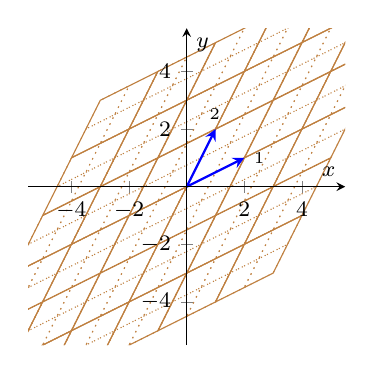
\begin{tikzpicture}
\begin{axis}[small,font=\footnotesize
  ,axis lines=middle, axis equal image, view={0}{90}
  ,xmax=5.5,ymax=5.5,xmin=-5.5,ymin=-5.5
  ,xlabel={$x$},ylabel={$y$}
  ]
\addplot3[mesh,brown,samples=13,domain=-3:3,dotted] (2*x+y,x+2*y,0);
\addplot3[mesh,brown,samples=7,domain=-3:3] (2*x+y,x+2*y,0);
\addplot[blue,quiver={u=2,v=1},-stealth,thick] coordinates {(0,0)};
\node[right] at (axis cs:2,1) {$\vv_1$};
\addplot[blue,quiver={u=1,v=2},-stealth,thick] coordinates {(0,0)};
\node[above] at (axis cs:1,2) {$\vv_2$};
\end{axis}
\end{tikzpicture}
\end{wrapfigure}
Now proceed to consider a general vector \((x,y)\) and seek it as a linear combination of~\(\vv_1\) and~\(\vv_2\), namely \((x,y)=c_1\vv_1+c_2\vv_2\)\,.
That is, let's write each and every point in the plane as a linear combination of~\(\vv_1\) and~\(\vv_2\) as illustrated to the right.
Rewrite the equation in matrix-vector form as
\begin{equation*}
\begin{bmatrix} \vv_1&\vv_2 \end{bmatrix}
\begin{bmatrix} c_1\\c_2 \end{bmatrix}
=\begin{bmatrix} x\\y \end{bmatrix}
,\quad\text{that is,}\quad
V\cv=\begin{bmatrix} x\\y \end{bmatrix}
\text{ for }V=\begin{bmatrix} 2&1\\1&2 \end{bmatrix}.
\end{equation*}
For any given \((x,y)\), \(V\cv=(x,y)\) is a system of linear equations for the coefficients~\cv.
\cref{thm:ftim2} asserts that the system has a unique solution~\cv\ if and only if the matrix~\(V\) is invertible.
Here the unique solution is then that the vector of coefficients
\begin{equation*}
\cv=V^{-1}\begin{bmatrix} x\\y \end{bmatrix}
=\begin{bmatrix} \frac23&-\frac13\\-\frac13&\frac23 \end{bmatrix}
\begin{bmatrix} x\\y \end{bmatrix}.
\end{equation*}
Equivalently, \cref{thm:ftim2iii} asserts the system has a unique solution~\cv---unique coefficients~\cv---if and only if the {homogeneous} system \(V\cv=\ov\) has only the zero solution \(\cv=\ov\)\,.
It is this last statement that leads to the upcoming \cref{def:lindep} of \idx{linearly independent} vectors.
\end{solution}
\end{example}
\endgroup



{%group
\def\temp{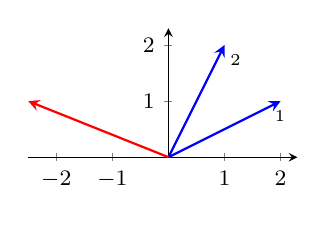
\begin{tikzpicture}
\begin{axis}[footnotesize,font=\footnotesize
  ,axis lines=middle, axis equal image
  ,xmax=2.3,ymax=2.3
  ]
\addplot[blue,quiver={u=2,v=1},-stealth,thick] coordinates {(0,0)};
\node[below] at (axis cs:2,1) {$\vv_1$};
\addplot[blue,quiver={u=1,v=2},-stealth,thick] coordinates {(0,0)};
\node[below] at (axis cs:1,2) {$\quad\vv_2$};
\addplot[red,quiver={u=-2.5,v=1},-stealth,thick] coordinates {(0,0)};
%\node[right] at (axis cs:-2.5,1) {$(-2.5,1)$};
\end{axis}
\end{tikzpicture}}
\begin{activity}[\temp]
The vector shown to the right is which of the following \idx{linear combination}s of shown vectors~\(\vv_1\) and~\(\vv_2\)?
\actposs{\(-2\vv_1 +1.5\vv_2\)}
{\(-2.5\vv_1 +2\vv_2\)}
{\(-1.5\vv_1 +\vv_2\)}
{\(-\vv_1 +\vv_2\)}
\end{activity}
}





\needlines8
\begin{wrapfigure}r{0pt}
\qview{113}{117}{\begin{tikzpicture}
\begin{axis}[small,font=\small
  ,xlabel={$x$}, ylabel={$y$}, zlabel={$z$},label shift={-2ex}
  ,no marks ,domain=-2.5:2.5,axis equal image,zmax=2.5,zmin=-2.5
  ,view={\q}{30}
  ] 
\addplot3[surf,blue,samples=3,opacity=0.3]  {-x-y};
\addplot3[blue,thick,quiver={u=-1,v=1,w=0},-stealth] coordinates {(0,0,0)};
\node[right] at (axis cs:-1,1,0) {$\vv_1$};
\addplot3[blue,thick,quiver={u=1,v=-2,w=1},-stealth] coordinates {(0,0,0)};
\node[below] at (axis cs:1,-2,1) {$\vv_2$};
\addplot3[blue,thick,quiver={u=0,v=1,w=-1},-stealth] coordinates {(0,0,0)};
\node[below] at (axis cs:0,1,-1) {$\vv_3$};
\end{axis}
\end{tikzpicture}}
\end{wrapfigure}
\begin{example}[3D failure] 
Show that vectors in~\(\RR^3\) are not written uniquely as a \idx{linear combination} of \(\vv_1=(-1,1,0)\), \(\vv_2=(1,-2,1)\), and \(\vv_3=(0,1,-1)\). 

One reason for the failure is that these three vectors only span a plane, as shown to the right in stereo.  
The solution here looks at the different issue of unique representation.

\begin{solution} 
As one example, consider the vector~\((1,0,-1)\):
\begin{eqnarray*}
(1,0,-1)&=&-1\vv_1+0\vv_2+1\vv_3\,;
\\(1,0,-1)&=&1\vv_1+2\vv_2+3\vv_3\,;
\\(1,0,-1)&=&-2\vv_1-1\vv_2+0\vv_3\,;
\\(1,0,-1)&=&(-1+t)\vv_1+t\vv_2+(1+t)\vv_3\,,\quad\text{for every }t.
\end{eqnarray*}
This last combination shows that there are an infinite number of ways to write \((1,0,-1)\) as a linear combination of~\(\vv_1\), \(\vv_2\), and~\(\vv_3\).
Such an infinity of linear combinations means that~\(\vv_1\), \(\vv_2\), and~\(\vv_3\) cannot form the basis for a useful `coordinate system' because we cannot easily distinguish between the different combinations all describing the same vector.
The reason for the infinity of combinations is that there is a nontrivial linear combination of~\(\vv_1\), \(\vv_2\), and~\(\vv_3\) which is zero, namely here \(\vv_1+\vv_2+\vv_3=\ov\)\,.
It is this last statement that leads to the \cref{def:lindep} of \text{\idx{linearly dependent} vectors.}
\end{solution}
\end{example}





\begin{definition} \label{def:lindep} 
A set of vectors \(\{\hlist\vv k\}\) is \bfidx{linearly dependent} if there are \idx{scalar}s \hlist ck, at least one of which is nonzero, such that \(\lincomb c\vv k=\ov\)\,.
A set of vectors that is not linearly dependent is called \bfidx{linearly independent} (characterized by \emph{only} the linear combination with \(c_1=c_2=\cdots=c_k=0\) gives the \text{\idx{zero vector}).}
\end{definition}

When reading the terms ``linearly in/dependent'' be very careful: it is all too easy to misread the presence or absence of the crucial ``in''~syllable. 
The presence or absence of the ``in''~syllable makes all the difference between the property and its opposite.


\begin{example} \label{eg:lindep}
Are the following sets of vectors linearly dependent or linearly independent.  Give reasons.
\begin{enumerate}[ref=\ref{eg:lindep}(\alph*)]
\item\label[example]{eg:lindepa} \(\{(-1,1,0),\ (1,-2,1),\ (0,1,-1)\}\) 
\begin{solution} 
The set is linearly dependent as the linear combination \((-1,1,0)+(1,-2,1)+(0,1,-1)=(0,0,0)\). 
\end{solution}

\item\label[example]{eg:lindepb} \(\{(2,1),\ (1,2)\}\) 
\begin{solution} 
The set is linearly independent because the linear combination equation \(c_1(2,1)+c_2(1,2)=(0,0)\) is equivalent to the homogeneous matrix-vector system \(\begin{bmat} 2&1\\1&2 \end{bmat}\cv=\ov\) which has \emph{only} the zero solution \(\cv=\ov\)\,. 
\end{solution}

%\item \(\{(-1,1,0),\ (1,-2,1)\}\)
%\begin{solution} 
%The set is linearly independent: for the linear combination \(c_1(-1,1,0)+c_2(1,-2,1)
%=(-c_1+c_2,c_1-2c_2,c_2)=\ov\) requires the last component to be zero which requires \(c_2=0\);
%then either of the other components requires \(c_1=0\)\,.
%\end{solution}

\item\label[example]{eg:lindepc} \(\{(-2,4,1,-1,0)\}\)
\begin{solution} 
This set of one vector in~\(\RR^5\) is linearly independent as \(c_1(-2,4,1,-1,0)=\ov\) can only be satisfied with \(c_1=0\)\,. 
Indeed, any one nonzero vector~\vv\ in~\(\RR^n\) forms a linearly independent set,~\(\{\vv\}\), for the same reason.
\end{solution}



\item \(\{(2,1),\ (0,0)\}\) 
\begin{solution} 
The set is linearly dependent because the linear combination  \(0(2,1)+c_2(0,0)=(0,0)\) for every nonzero~\(c_2\). 
\end{solution}


\item \(\{\ov,\hlist[2]\vv k\}\)
\begin{solution} 
Every  set that includes the zero vector is linearly dependent as
\(c_1\ov+0\vv_2+\cdots+0\vv_k=\ov\) for every nonzero~\(c_1\).
\end{solution}

\item \index{e@$\ev_j$}\(\{\ev_1,\ev_2,\ev_3\}\), the set of \idx{standard unit vector}s in~\(\RR^3\).
\begin{solution} 
This set is linearly independent as
\(c_1\ev_1+c_2\ev_2+c_3\ev_3=(c_1,c_2,c_3)=\ov\)
\emph{only} when all three components are zero, \(c_1=c_2=c_3=0\)\,. 
\end{solution}

\item \(\{(\frac13,\frac23,\frac23),\ (\frac23,\frac13,-\frac23)\}\)
\begin{solution} 
This set is linearly independent.
Seek some linear combination \(c_1(\frac13,\frac23,\frac23) +c_2(\frac23,\frac13,-\frac23) =\ov\)\,.
Take the dot product of both sides of this equation with \((1,2,2)\):
\begin{eqnarray*}
&&c_1\begin{bmatrix}\frac13\\\frac23\\\frac23 \end{bmatrix}\cdot\begin{bmatrix} 1\\2\\2 \end{bmatrix} +c_2\begin{bmatrix} \frac23\\\frac13\\-\frac23 \end{bmatrix}\cdot\begin{bmatrix} 1\\2\\2 \end{bmatrix} =\ov\cdot\begin{bmatrix} 1\\2\\2 \end{bmatrix}
\\\implies&& c_13+c_20=0
\implies c_1=0\,.
\end{eqnarray*}
Also, take the dot product with \((2,1,-2)\): 
\begin{eqnarray*}
&&c_1\begin{bmatrix}\frac13\\\frac23\\\frac23 \end{bmatrix}\cdot\begin{bmatrix} 2\\1\\-2 \end{bmatrix} +c_2\begin{bmatrix} \frac23\\\frac13\\-\frac23 \end{bmatrix}\cdot\begin{bmatrix} 2\\1\\-2 \end{bmatrix} =\ov\cdot\begin{bmatrix} 2\\1\\-2 \end{bmatrix}
\\\implies&& c_10+c_23=0
\implies c_2=0\,.
\end{eqnarray*}
Hence \(c_1=c_2=0\) is the \emph{only} possibility and so the two given vectors are linearly independent.
\end{solution}

\end{enumerate}
These last two cases generalize to the next \cref{thm:ortholi} about the linear independence of every \idx{orthonormal set} of vectors.
\end{example}



\begin{activity}
Which of the following sets of vectors is linearly independent?
\actposs{\(\{(-1,1),(0,1)\}\)}
{\(\{(0,0),(-2,1)\}\)}
{\(\{(0,1),(0,-1)\}\)}
{\(\{(-1,2),(-2,4)\}\)}
\end{activity}




\begin{example}[calculus extension] 
In calculus the notion of a function corresponds to the notion of a vector in our linear algebra.  
For the purposes of this example, consider `vector' and `function' to be synonymous, and that `all \idx{components}' and `all~\(x\)' are synonymous. 
Show that the set \(\{e^x,e^{-x},\cosh x,\sinh x\}\) is linearly dependent.  
What is a subset that is \text{linearly independent?}
\begin{solution} 
The definition of the hyperbolic functions, namely that \(\cosh x=(e^x+e^{-x})/2\) and \(\sinh x=(e^x-e^{-x})/2\), immediately gives two nontrivial linear combinations that are zero for all~\(x\), namely \(2\cosh x-e^x-e^{-x}=0\) and \(2\sinh x-e^x+e^{-x}=0\) for all~\(x\).
Either one of these implies that the set \(\{e^x,e^{-x},\cosh x,\sinh x\}\) is \text{linearly dependent.}

Because \(e^x\) and~\(e^{-x}\) are not proportional to each other, there is no linear combination which is zero for all~\(x\), and hence the set \(\{e^x,e^{-x}\}\) is linearly independent (as are any other pairs of the four functions).
\end{solution}
\end{example}







\begin{theorem} \label{thm:ortholi}
Every \idx{orthonormal set} of vectors (\cref{def:orthoset}) is \idx{linearly independent}.
\end{theorem}
\begin{proof} %Take dot products with the defining equation.
Let \(\{\hlist\vv k\}\) be an orthonormal set of vectors in~\(\RR^n\).
Let's find all possible scalars \hlist ck such that \(\lincomb c\vv k=\ov\)\,.
Taking the dot product of this equation with~\(\vv_1\) requires
\(c_1\vv_1\cdot\vv_1+c_2\vv_2\cdot\vv_1+\cdots+c_k\vv_k\cdot\vv_1=\ov\cdot\vv_1\)\,;
by orthonormality this equation becomes
\(c_11+c_20+\cdots+c_k0=0\)\,; that is, \(c_1=0\)\,.
Similarly, taking the dot product with~\(\vv_2\) requires
\(c_1\vv_1\cdot\vv_2+c_2\vv_2\cdot\vv_2+\cdots+c_k\vv_k\cdot\vv_2=\ov\cdot\vv_2\)\,;
by orthonormality this equation becomes
\(c_10+c_21+\cdots+c_k0=0\)\,; that is, \(c_2=0\)\,.
And so on for every vector in the set, implying the coefficients \(c_1=c_2=\cdots=c_k=0\) is the only possibility.
By \cref{def:lindep}, the orthonormal set must be \text{linearly independent.}
\end{proof}


In contrast to orthonormal vectors which are always linearly independent, a set of two vectors proportional to each other is always linearly dependent as seen in the following examples.
This linear dependence of proportional vectors then generalizes in the forthcoming \cref{thm:lindeplc}.




\begin{example} 
Show that the following sets are linearly dependent.
\begin{enumerate}
\item \(\{(1,2),\ (3,6)\}\)
\begin{solution} 
Since \((3,6)=3(1,2)\) then the linear combination \(1(3,6)-3(1,2)=\ov\) and the set is linearly dependent. 
\end{solution}

\item \(\{(2.2,-2.1,0,1.5),\ (-8.8,8.4,0,-6)\}\)
\begin{solution} 
Since  \((-8.8,8.4,0,-6)=-4(2.2,-2.1,0,1.5)\) then the linear combination 
\begin{equation*}
(-8.8,8.4,0,-6)+4(2.2,-2.1,0,1.5)=\ov\,,
\end{equation*}
and so the set is linearly dependent.
\end{solution}
\end{enumerate}
\end{example}




\begin{activity}
For what value of~\(c\) is the set \(\{(-3c,-2+2c),(1,2)\}\) linearly dependent?
%v=round(randn(2)*2)+0,w=round(randn(2))+0,0-eig(v,w)
\actposs[4]{\(c=\frac14\)}{\(c=-\frac13\)}{\(c=0\)}{\(c=1\)}
\end{activity}




\begin{theorem} \label{thm:lindeplc} 
A set of vectors \(\{\hlist\vv m\}\) is \idx{linearly dependent} if and only if at least one of the vectors can be expressed as a \idx{linear combination} of the other vectors.
In particular, a set of two vectors \(\{\vv_1,\vv_2\}\) is linearly dependent if and only if one of the vectors is a scalar multiple of \text{the other.}
\end{theorem}

\begin{proof} 
\cref{ex:lindeplc} establishes the particular case of a set of two vectors.
%Start with the particular case of the set of two vectors \(\{\vv_1,\vv_2\}\).
%Say \(\vv_1\) is a multiple of~\(\vv_2\), \(\vv_1=c\vv_2\)\,, then the linear combination \(\vv_1-c\vv_2=\ov\)\,, and so the set is linearly dependent. 
%Similarly if \(\vv_2\) is a multiple of~\(\vv_1\).
%Conversely, if the set is linearly dependent then \(c_1\vv_1+c_2\vv_2=0\) where one or both of \(c_1,c_2\neq0\): if \(c_1\neq 0\) then rearrange to \(\vv_1=-(c_2/c_1)\vv_2\) and so \(\vv_1\) is a multiple of~\(\vv_2\); and similarly if \(c_2\neq 0\)\,.

In the general case of \(m\)~vectors, first establish that if one of the vectors can be expressed as a {linear combination} of the others, then the set is linearly dependent.
Let's label the set of vectors so that it is vector~\(\vv_1\) which is a linear combination of the others; that is, \(\vv_1=\lincomb[2]c\vv m\)\,.
Rearranging, \((-1)\vv_1+\lincomb[2]c\vv m=\ov\)\,; that is, there is a non-trivial (as at least \(c_1=-1\neq0\)) linear combination of the set of vectors which is zero.
Hence the set is \text{linearly dependent.}

Second, establish the converse.  
Given the set is linearly dependent, there exist coefficients, not all zero, such that \(\lincomb c\vv m=\ov\)\,.  
Suppose that we have labelled the vectors so that \(c_1\neq 0\)\,.  
Then rearranging the equation gives
\(c_1\vv_1=-c_2\vv_2-c_3\vv_3-\cdots-c_m\vv_m\)\,.
Divide by the nonzero~\(c_1\) to deduce
\(\vv_1=-(c_2/c_1)\vv_2-(c_3/c_1)\vv_3-\cdots-(c_m/c_1)\vv_m\)\,;
that is, \(\vv_1\)~is a linear combination of the \text{other vectors.}
\end{proof}


\begin{example} 
Invoke \cref{thm:lindeplc} to deduce whether the following sets are linearly independent or linearly dependent.
\begin{enumerate}
\item \(\{(-1,1,0),\ (1,-2,1),\ (0,1,-1)\}\)
\begin{solution} 
Since \((1,-2,1)=-(-1,1,0)-(0,1,-1)\) the set must be linearly dependent.
\end{solution}

\item 
\begin{figbox}{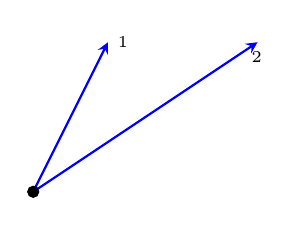
\begin{tikzpicture}
\begin{axis}[footnotesize,font=\footnotesize
  ,axis lines=none, axis equal image
  ]
\addplot[blue,quiver={u=3,v=2},-stealth,thick] coordinates {(0,0)};
\node[below] at (axis cs:3,2) {$\vv_2$};
\addplot[blue,quiver={u=1,v=2},-stealth,thick] coordinates {(0,0)};
\node[right] at (axis cs:1,2) {$\vv_1$};
\addplot[black,mark=*] coordinates {(0,0)};
\end{axis}
\end{tikzpicture}}%
The set of two vectors shown to the right.

\begin{solution} 
Since the two vectors are not proportional to each other, we cannot write either as a scalar multiple of the other, and so the pair are linearly independent. 

\end{solution}
\end{figbox}


\item 
\begin{figbox}{\begin{tikzpicture}
\begin{axis}[footnotesize,font=\footnotesize
  ,axis lines=none, axis equal image
  ]
\addplot[blue,quiver={u=3,v=2},-stealth,thick] coordinates {(0,0)};
\node[below] at (axis cs:3,2) {$\vv_2$};
\addplot[blue,quiver={u=-1,v=-0.667},-stealth,thick] coordinates {(0,0)};
\node[above] at (axis cs:-1,-0.667) {$\vv_1$};
\addplot[black,mark=*] coordinates {(0,0)};
\end{axis}
\end{tikzpicture}}%
The set of two vectors shown to the right.

\begin{solution} 
Since the two vectors appear proportional to each other, \(\vv_2\approx (-3)\vv_1\)\,,  so the pair appear linearly dependent. 

\end{solution}
\end{figbox}



\item \(\{(1,3,0,-1),\ (1,0,-4,2),\ (-2,3,0,-3),\ (0,6,-4,-2)\}\)
\begin{solution} 
Notice that the last vector is the sum of the first three, \((0,6,-4,-2)=(1,3,0,-1)+(1,0,-4,2)+(-2,3,0,-3)\), and so the set is linearly dependent. 
\end{solution}


\end{enumerate}
\end{example}




Recall that \cref{thm:orthoevec} established that for every two distinct {eigenvalue}s of a symmetric matrix~\(A\), any corresponding two {eigenvector}s are {orthogonal}.
Consequently, for a symmetric matrix~\(A\), a set of eigenvectors from distinct eigenvalues forms an \idx{orthogonal set}.
The following \cref{thm:indepev} generalizes this property to non-symmetric matrices using the concept of linear independence.
That the corresponding eigenvalues are all different \text{is crucial.}


\begin{theorem} \label{thm:indepev}
For every \(n\times n\) matrix~\(A\), let \hlist\lambda m\ be \idx{distinct eigenvalues} of~\(A\) with corresponding \idx{eigenvector}s \hlist\vv m.
Then the set \(\{\hlist \vv m\}\) is \idx{linearly independent}.
\end{theorem}
\begin{proof} 
Use \idx{contradiction}.
Assume the set \(\{\hlist \vv m\}\) is linearly dependent.
Choose~\(k<m\) such that the set \(\{\hlist\vv k\}\) is linearly independent, whereas the set \(\{\hlist\vv{k+1}\}\) is linearly dependent.
Hence there exists non-trivial coefficients such that 
\begin{equation*}
\lincomb c\vv{k}+c_{k+1}\vv_{k+1}=\ov\,;
\end{equation*}
further, \(c_{k+1}\neq0\) as \(\{\hlist\vv k\}\) is linearly independent.
Pre-multiply the linear combination by matrix~\(A\):
\begin{eqnarray*}&&
\lincomb c{A\vv}k+c_{k+1}A\vv_{k+1}=A\ov
\\\implies&&
c_1\lambda_1\vv_1+c_2\lambda_2\vv_2+\cdots+c_k\lambda_k\vv_k+c_{k+1}\lambda_{k+1}\vv_{k+1}=\ov\,.
\end{eqnarray*}
Now subtract \(\lambda_{k+1}\times\) the original linear combination:
\begin{eqnarray*}&&
\phantom{{}+(}c_1\lambda_1\vv_1+c_2\lambda_2\vv_2+\cdots+c_k\lambda_k\vv_k+c_{k+1}\lambda_{k+1}\vv_{k+1}
\\&&{}
-\left(\lincomb c{\lambda_{k+1}\vv}{k}
+c_{k+1}\lambda_{k+1}\vv_{k+1}\right)=\ov
\\\implies&&
c_1(\lambda_1-\lambda_{k+1})\vv_1+c_2(\lambda_2-\lambda_{k+1})\vv_2+\cdots
\\&&{}
+c_k(\lambda_k-\lambda_{k+1})\vv_k
+c_{k+1}\underbrace{(\lambda_{k+1}-\lambda_{k+1})}_{=0}\vv_{k+1}=\ov
\\\implies&&
\lincomb{c'}\vv k=\ov
\end{eqnarray*}
for coefficients \(c'_j=c_j(\lambda_j-\lambda_{k+1})\).
Since all the eigenvalues are distinct, \(\lambda_j-\lambda_{k+1}\neq0\)\,, and since the coefficients~\(c_j\) are not all zero, hence \(c'_j\)~are not all zero.
Thus we have created a non-trivial linear combination of \hlist \vv k\ which is zero, and so the set \(\{\hlist\vv k\}\) is linearly dependent.
This contradiction of the choice of~\(k\) proves that the assumption must be wrong.
Hence the set \(\{\hlist \vv m\}\) is linearly independent, \text{as required.}
\end{proof}



\begin{activity}
The matrix \(\begin{bmatrix} 2&1\\a^2&2 \end{bmatrix}\) has \idx{eigenvector}s proportional to~\((1,a)\), and proportional to~\((1,-a)\).
For what values of~\(a\) does the matrix have two \idx{distinct eigenvalues}?
\actposs[4]{\(a\neq0\)}{\(a\neq-1\)}{\(a\neq1\)}{\(a\neq2\)}
\end{activity}






\begin{example} \label{eg:indepev}
For each of the following matrices, show that the \idx{eigenvector}s from \idx{distinct eigenvalues} form linearly independent sets.
\begin{enumerate}[ref=\ref{eg:indepev}(\alph*)]
\item  Consider the matrix \(B=\begin{bmat}-1&1&-2
\\-1&0&-1
\\0&-3&1 \end{bmat}\) from \cref{eg:faespm}.
\begin{solution} \sloppy
In \script, executing 
\begin{verbatim}
B=[-1 1 -2
 -1 0 -1
 0 -3 1]
[V,D]=eig(B)
\end{verbatim}
\setbox\ajrqrbox\hbox{\qrcode{% eigenvectors
B=[-1 1 -2
 -1 0 -1
 0 -3 1]
[V,D]=eig(B)
}}%
\marginajrbox%
gives eigenvectors and corresponding eigenvalues in
\begin{verbatim}
V =
    -0.5774     0.7071    -0.7071
    -0.5774     0.0000     0.0000
    -0.5774    -0.7071     0.7071
D =
         -2          0          0
          0          1          0
          0          0          1
\end{verbatim} 
Recognizing \(0.7071=1/\sqrt2\)\,, the last two eigenvectors, \((1/\sqrt2,0,-1/\sqrt2)\) and  \((-1/\sqrt2,0,1/\sqrt2)\), form a linearly dependent set because they are proportional to each other.
This linear dependence does not confound  \cref{thm:linhomo} because the corresponding eigenvalues are the same, not distinct, namely \(\lambda=1\)\,.
The theorem only applies to eigenvectors of \text{distinct eigenvalues.}

Here the two distinct eigenvalues are \(\lambda=-2\) and \(\lambda=1\)\,.
Recognizing \(0.5774=1/\sqrt3\)\,, two corresponding eigenvectors are \((-1/\sqrt3,-1/\sqrt3,-1/\sqrt3)\) and \((1/\sqrt2,0,-1/\sqrt2)\).
Because the zero component in the second corresponds to a nonzero component in the first, these cannot be proportional to each other, and so the pair form a linearly \text{independent set.}
\end{solution}


\item\label[example]{eg:indepeva} \cref{eg:fiveev} found the eigenvalues and eigenvectors of matrix
\begin{equation*}
A=\begin{bmatrix}0&3&0&0&0
\\1&0&3&0&0
\\0&1&0&3&0
\\0&0&1&0&3
\\0&0&0&1&0\end{bmatrix}
\end{equation*}
In \script\ execute
\begin{verbatim}
A=[0 3 0 0 0
 1 0 3 0 0
 0 1 0 3 0
 0 0 1 0 3
 0 0 0 1 0]
[V,D]=eig(A)
\end{verbatim}
\setbox\ajrqrbox\hbox{\qrcode{% eigenvectors
A=[0 3 0 0 0
 1 0 3 0 0
 0 1 0 3 0
 0 0 1 0 3
 0 0 0 1 0]
[V,D]=eig(A)
svd(V)
}}%
\marginajrbox%
to obtain the report \twodp
\begin{verbatim}
V =
   0.62  -0.62   0.94  -0.85  -0.85
   0.62   0.62  -0.00   0.49  -0.49
   0.42  -0.42  -0.31  -0.00   0.00
   0.21   0.21  -0.00  -0.16   0.16
   0.07  -0.07   0.10   0.09   0.09
D =
   3.00      0      0      0      0
      0  -3.00      0      0      0
      0      0  -0.00      0      0
      0      0      0  -1.73      0
      0      0      0      0   1.73
\end{verbatim}
The five eigenvalues are all distinct, so \cref{thm:linhomo} asserts that a set of corresponding eigenvectors is linearly independent.
The five columns of~\(V\), call them \hlist\vv5, are a set of corresponding eigenvectors.

To confirm their linear independence let's seek a linear combination being zero, that is, \(\lincomb c\vv5=\ov\)\,.
Written as a matrix-vector system we seek \(\cv=(\hlist c5)\) such that \(V\cv=\ov\)\,.
Because the five singular values of square matrix~\(V\) are all nonzero,\footnote{One could alternatively compute the determinant \(\texttt{det(V)}=0.09090\) and because it is nonzero \cref{thm:ftim3} asserts that the equation has only the solution \(\cv=\ov\)\,.} obtained from \verb|svd(V)|~as
\begin{verbatim}
ans =
   1.7703
   1.1268
   0.6542
   0.3625
   0.1922
\end{verbatim}
consequently \cref{thm:ftim2} asserts that \(V\cv=\ov\) has only the zero solution.
Hence, by \cref{def:lindep} the set of eigenvectors in the columns of~\(V\) is linearly independent. 

\end{enumerate}
\end{example}


This last case of the preceding \cref{eg:indepeva} connects the concept of linear in/dependence to the existence or otherwise of nonzero solutions to a homogeneous system of \idx{linear equation}s, \(V\cv=\ov\)\,.
So does \cref{eg:lindepb}.
The great utility of this connection is that we understand a lot about homogeneous \idx{system}s of linear equations.
The next \cref{thm:linhomo} establishes this connection \text{in general.}


\begin{theorem} \label{thm:linhomo} 
Let \hlist\vv m\ be vectors in~\(\RR^n\),
and let the \(n\times m\) matrix \(V=\begin{bmatrix} \vv_1&\vv_2&\cdots&\vv_m \end{bmatrix}\).  
Then the set \(\{\hlist\vv m\}\) is \idx{linearly dependent} if and only if the \idx{homogeneous} \idx{system} \(V\cv=\ov\) has a nonzero solution~\cv.
\end{theorem}
\begin{proof} 
Now \(\{\hlist\vv m\}\) is \idx{linearly dependent} if and only if there are scalars, not all zero, such that the equation \(\lincomb c\vv m=\ov\) holds (\cref{def:lindep}).
Let the vector \(\cv=(\hlist cm)\), then this equation is equivalent to the statement \(V\cv=\ov\)\,.
That is, if and only if \(V\cv=\ov\) has a \text{nonzero solution.}
\end{proof}





Recall \cref{thm:orthcomp}, that in~\(\RR^n\) there can be no more that \(n\)~vectors in an \idx{orthogonal set} of vectors.
The following theorem is the generalization: in~\(\RR^n\) there can be no more than \(n\)~vectors in a linearly independent set of vectors.

\begin{activity}
Which of the following sets of vectors are linearly dependent?
\def\temp#1{\begin{tikzpicture}
\begin{axis}[footnotesize,font=\footnotesize
  ,axis lines=none, axis equal image
  ,xmax=2,ymax=1,xmin=-0.55,ymin=-1.5
  ]
\addplot[blue,quiver={u=2,v=1},-stealth,thick,mark=*] coordinates {(0,0)};
\ifnum#1>1\addplot[blue,quiver={u=-0.4,v=1},-stealth,thick] coordinates {(0,0)};\fi
\ifnum#1>2\addplot[blue,quiver={u=-0.5,v=-1.5},-stealth,thick] coordinates {(0,0)};\fi
\end{axis}
\end{tikzpicture}}
\actposs{\temp3}{\temp1}{\temp2}{None of these sets.}
\end{activity}



\begin{theorem} \label{thm:mgtnli} 
Every  set of \(m\)~vectors in~\(\RR^n\) is \idx{linearly dependent} when the number of vectors \(m>n\)\,.
\end{theorem}
\begin{proof} 
Form the \(m\)~vectors \(\hlist\vv m\in\RR^n\)\ into the \(n\times m\) matrix \(V=\begin{bmatrix} \vv_1&\vv_2&\cdots&\vv_m \end{bmatrix}\).
Consider the homogeneous system \(V\cv=\ov\)\,: 
%it has nonzero solutions iff the nullspace has nonzero dimension (\cref{thm:homosubsp}).
%Recall (\cref{def:nullity}) that the dimension of the nullspace is the nullity, and the Rank \cref{thm:rank} gives
%\begin{eqnarray*}
%\nullity A&=&m-\rank A
%\quad(\text{as \(m\) is the number of columns})
%\\&\geq&m-n
%\quad(\text{as }\rank A\leq \min(m,n)=n\text{ here})
%\\&>&0\quad(\text{again as }m>n\text{ here}).
%\end{eqnarray*}
as \(m>n\)\,, \cref{thm:feweqns} (with the meaning of \(m\) and~\(n\) swapped) asserts that \(V\cv=\ov\) has infinitely many solutions.
Thus \(V\cv=\ov\) has nonzero solutions, so \cref{thm:linhomo} implies that the set of eigenvectors \(\{\hlist\vv m\}\) is \text{linearly dependent.}
\end{proof}



\begin{example} 
%Use \cref{thm:linhomo} and \cref{thm:mgtnli}
Determine if the following sets of vectors are linearly dependent or independent.  Give reasons.

\begin{enumerate}
\item \(\{(-1,-2)\clb (-1,4)\clb (0,5)\clb (2,3)\}\)
\begin{solution} 
As there are four vectors in~\(\RR^2\) so \cref{thm:mgtnli} asserts the set is linearly dependent.
\end{solution}

\item \(\{(-6,-4,-1,-2)\clb (2,0,1,-2)\clb (2,-1,-1,1)\}\)
\begin{solution} 
In \script\ form the matrix with these vectors as columns
\begin{verbatim}
V=[-6   2   2
  -4   0  -1
  -1   1  -1
  -2  -2   1]
svd(V)
\end{verbatim}
\setbox\ajrqrbox\hbox{\qrcode{% lin indep
V=[-6   2   2
  -4   0  -1
  -1   1  -1
  -2  -2   1]
svd(V)
}}%
\marginajrbox%
and find that the three singular values are all nonzero (namely \(7.7568\), \(2.7474\), and~\(2.2988\)).
Hence there are \emph{no} free variables when solving \(V\cv=\ov\) (\cref{pro:gensol}), and consequently there is only the unique solution \(\cv=\ov\)\,.
By \cref{thm:linhomo}, the set of vectors is \text{linearly independent.}
\end{solution}

\item \(\{(-1,-2,2,-1)\clb (1,3,1,-1)\clb (-2,-4,4,-2)\}\)
\begin{solution} 
By inspection, the third vector is twice the first.
Hence the linear combination \(2(-1,-2,2,-1)+0(1,3,1,-1)-(-2,-4,4,-2)=\ov\) and so the set of vectors is linearly dependent. 
\end{solution}


\item \(\{(3,3,-1,-1)\clb (0,-3,-1,-7)\clb (1,2,0,2)\}\)
\begin{solution} 
In \script\ form the matrix with these vectors as columns
\begin{verbatim}
V=[3   0   1
   3  -3   2
  -1  -1   0
  -1  -7   2]
svd(V)
\end{verbatim}
\setbox\ajrqrbox\hbox{\qrcode{% lin indep
V=[3   0   1
   3  -3   2
  -1  -1   0
  -1  -7   2]
svd(V)
}}%
\marginajrbox%
and find that the three singular values are \(8.1393\), \(4.6638\), and~\(0.0000\).
The zero singular value implies that there is a free variable when solving \(V\cv=\ov\) (\cref{pro:gensol}), and consequently that there are infinitely many nonzero~\cv\ that solve \(V\cv=\ov\).
By \cref{thm:linhomo}, the set of vectors is \text{linearly dependent.}
\end{solution}

\item \(\{(10,3,3,1)\clb ( 2,-3,0,-1)\clb ( 1,-1,2,-1)\clb ( 2,-1,-3,0)\clb (-2,0,2,-1)\}\)
\begin{solution} 
There are five vectors in~\(\RR^4\) so \cref{thm:mgtnli} asserts that the set is linearly dependent.
\end{solution}




\item \(\sloppy\{(-0.4,-1.8,-0.2, 0.7,-0.2)\clb (-1.1, 2.8, 2.7,-3.0,-2.6)\clb (-2.3,-2.3, 4.1, 3.4,-1.6)\clb (-2.6,-5.3,-3.3,-1.3,-4.1)\clb ( 1.4, 5.2,-6.9,-0.7, 0.6)\}\)
\begin{solution} 
In \script\ form the matrix~\(V\) with these vectors as columns
\begin{verbatim}
V=[-0.4 -1.1 -2.3 -2.6 1.4
  -1.8  2.8 -2.3 -5.3  5.2
  -0.2  2.7  4.1 -3.3 -6.9
   0.7 -3.0  3.4 -1.3 -0.7
  -0.2 -2.6 -1.6 -4.1  0.6]
svd(V)
\end{verbatim}
\setbox\ajrqrbox\hbox{\qrcode{% lin indep
V=[-0.4 -1.1 -2.3 -2.6 1.4
  -1.8  2.8 -2.3 -5.3  5.2
  -0.2  2.7  4.1 -3.3 -6.9
   0.7 -3.0  3.4 -1.3 -0.7
  -0.2 -2.6 -1.6 -4.1  0.6]
svd(V)
}}%
\marginajrbox%
and find that the five singular values are \(10.6978\), \(8.0250\), \(5.5920\), \(3.0277\), and~\(0.0024\).
As the singular values are all nonzero, the homogeneous system \(V\cv=\ov\) has the unique solution \(\cv=\ov\) (\cref{pro:gensol}), and hence the set of five vectors are \text{linearly independent.}

However, the answer depends upon the context.  
In the strict mathematical context the vectors are unequivocally linearly independent.
But in the context of practical problems, where errors in matrix entries are likely, there are `shades of grey'. 
Here, one of the singular values is quite small, namely~\(0.0024\).
If the context informs us that the entries in the matrix had errors of say~\(0.01\), then this singular value is effectively zero (\cref{sec:rle}).
In the context of such errors, this set of five vectors would be  \text{linearly dependent.}
\end{solution}


\end{enumerate}
%for i=1:9999, a=round(randn(3,4)*3);if min(svd(a))<1e-7,null(a'),break,end,end
\end{example}













\subsection{Form a basis for subspaces}
\index{basis|(}
\index{subspace|(}


Recall that \cref{sec:lcss,sec:sbd} defined \idx{subspace}s and the \idx{span}, namely that a subspace is 
a set of vectors \idx{closed} under addition and \idx{scalar multiplication}, and a span gives a subspace as all \idx{linear combination}s of a set of vectors.
Also, \cref{def:orthobasis} defined an ``\idx{orthonormal basis}'' for a subspace to be a set of orthonormal vectors that span the subspace.
This section generalizes the concept of an ``orthonormal basis'' by relaxing the requirement of orthonormality to result in the concept of \text{a ``basis''.}


\begin{definition} \label{def:basis} 
A \bfidx{basis} for a \idx{subspace}~\WW\ of~\(\RR^n\) is a set of  vectors such that the set both \idx{span}s~\WW\ and is \idx{linearly independent}.
\end{definition}

\begin{example} 
\begin{enumerate}
\item Recall that \cref{eg:lindepb,eg:2dnoc} showed that the two vectors \((2,1)\) and \((1,2)\) are linearly independent and span~\(\RR^2\). 
Hence the set \(\{(2,1)\clb (1,2)\}\) is a basis of~\(\RR^2\).

\item Recall that \cref{eg:lindepa} showed that the set \(\{(-1,1,0)\clb (1,-2,1)\clb (0,1,-1)\}\) is linearly dependent, so this set cannot be a basis.

However, remove one vector from the set, such as the middle one, and consider the set \(\{(-1,1,0)\clb (0,1,-1)\}\).
As the two vectors are not proportional to each other, this set is linearly independent (\cref{thm:lindeplc}).
Also, the plane \(x+y+z=0\) is a subspace, say~\WW.
The plane~\WW\ is characterized by \(y=-x-z\)\,.
So every vector in~\WW\ can be written as \((x,-x-z,z)=(x,-x,0)+(0,-z,z)=(-x)(-1,1,0)+(-z)(0,1,-1)\). 
That is, \(\Span\{(-1,1,0)\clb (0,1,-1)\}=\WW\).
Hence \(\{(-1,1,0)\clb (0,1,-1)\}\) is a basis for the plane~\WW.

\item 
\begin{figbox}{\qview{30}{34} {\begin{tikzpicture}
\begin{axis}[small,font=\footnotesize, view={\q}{30}
  ,xlabel={$x$}, ylabel={$y$}, zlabel={$z$},label shift={-2ex}
  ,domain=-2:2,axis equal image
  ] 
\addplot3[blue,samples=3,no marks]  ({2.1*x},{1.3*x},{-1.1*x});
\addplot3[blue,thick,quiver={u=2.1,v=1.3,w=-1.1},-stealth,mark=*] coordinates {(0,0,0)};
\node[below] at (axis cs:2.1,1.3,-1.1) {$(2.1,1.3,-1.1)$};
\end{axis}
\end{tikzpicture}}}%
Find a basis for the line given parametrically as \(x=2.1t\)\,, \(y=1.3t\), and \(z=-1.1t\) (shown to the right in stereo).

\begin{solution} 
The vectors in the line may be written as \(\xv=(x,y,z) =(2.1t,1.3t,-1.1t) =(2.1,1.3,-1.1)t\)\,.
Since the parameter~\(t\) may vary over all values, vectors in the line form \(\Span\{(2.1,1.3,-1.1)\}\). 
Since \(\{(2.1,1.3,-1.1)\}\) is a linearly independent set of vectors (\cref{eg:lindepc}), it thus forms a basis for the vectors in the \text{given line.}

\end{solution}
\end{figbox}



\item 
\begin{figbox}{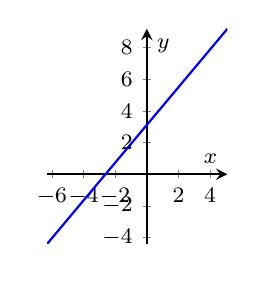
\begin{tikzpicture}
\begin{axis}[footnotesize,font=\footnotesize
  ,axis lines=middle, axis equal image
  ,xlabel={$x$}, ylabel={$y$}
  ,thick,no marks,samples=3 ,domain=-1:1 ] 
\addplot  ({5.7*x-0.6},{6.8*x+2.4});
\end{axis}
\end{tikzpicture}}%
Find a basis for the line given parametrically as \(x=5.7t-0.6\) and \(y=6.8t+2.4\)\,.

\begin{solution} 
The vectors in the line may be written as \(\xv=(5.7t-0.6,6.8t+2.4)\)\,.
But this does not form a subspace as it does not include the zero vector~\ov\ (as illustrated to the right). 
%the \(x\)-component is only zero for some positive~\(t\) whereas the \(y\)-component is only zero for some negative~\(t\) so they are never zero for the same value of parameter~\(t\).
Since this line is not a subspace, it cannot have a basis.


\end{solution}
\end{figbox}




\item 
\begin{figbox}{\qview{30}{34} {\begin{tikzpicture}
\begin{axis}[footnotesize,font=\footnotesize, view={\q}{30}
  ,xlabel={$x$}, ylabel={$y$}, zlabel={$z$},label shift={-2ex}
  ,no marks ,domain=-2:2 ] 
\addplot3[surf,blue,samples=3,opacity=0.3]  {-3*x+2*y};
\addplot3[blue,thick,quiver={u=1,v=0,w=-3},-stealth] coordinates {(0,0,0)};
\node[below] at (axis cs:1,0,-3) {$(1,0,-3)$};
\addplot3[blue,thick,quiver={u=0,v=1,w=2},-stealth] coordinates {(0,0,0)};
\node[above] at (axis cs:0,1,2) {$(0,1,2)$};
\end{axis}
\end{tikzpicture}}}%
Find a basis for the plane \(3x-2y+z=0\)\,.

\begin{solution} 
Writing the equation of the plane as \(z=-3x+2y\) we then write the plane parametrically (\cref{sec:nvep}) as the vectors \(\xv=(x,y,-3x+2y) =(x,0,-3x)+(0,y,2y) =x(1,0,-3) +y(0,1,2)\).
Since \(x\) and~\(y\) may vary over all values, the plane is the subspace \(\Span\{(1,0,-3)\clb (0,1,2)\}\) (as illustrated above-right in stereo).
Since \((1,0,-3)\) and \((0,1,2)\) are not proportional to each other, they form a linearly independent set.
Hence \(\{(1,0,-3)\clb (0,1,2)\}\) is a basis for \text{the plane.}

\end{solution}
\end{figbox}





\item %keep this as the last case of this example
Prove that every \idx{orthonormal basis} of a subspace~\WW\ is also a basis of~\WW.
\begin{solution} 
\cref{thm:ortholi} establishes that every orthonormal basis is linearly independent.
By \cref{def:orthobasis}, an orthonormal basis of~\WW\ spans~\WW.
Hence an orthonormal basis of~\WW\ is also a basis of~\WW.
\end{solution}
\end{enumerate}
\end{example}




\begin{activity}
Which of the following sets of vectors forms a basis for~\(\RR^2\), but is not an \idx{orthonormal basis} for~\(\RR^2\)?
\def\temp#1{\begin{tikzpicture}
\begin{axis}[footnotesize,font=\footnotesize
  ,axis lines=none, axis equal image
  ,xmax=1,ymax=2,xmin=-2,ymin=-1.3
  ]
\addplot[blue,quiver={u=1,v=2},-stealth,thick,mark=*] coordinates {(0,0)};
\ifnum#1=2\addplot[blue,quiver={u=-2,v=1},-stealth,thick] coordinates {(0,0)};\fi
\ifnum#1>2\addplot[blue,quiver={u=0.7,v=-1.3},-stealth,thick] coordinates {(0,0)};\fi
\ifnum#1>3\addplot[blue,quiver={u=-2,v=-0.5},-stealth,thick] coordinates {(0,0)};\fi
\end{axis}
\end{tikzpicture}}
\actposs[4]{\temp3}{\temp1}{\temp2}{\temp4}
\end{activity}






Recall that \cref{thm:sameD} establishes that an \idx{orthonormal basis} of a given subspace always has the same number of vectors.
The following theorem establishes that the same is true for general bases.
The proof directly generalizes that for \cref{thm:sameD}.

\begin{theorem} \label{thm:sameDii} 
Every basis for a given \idx{subspace} has the same number of vectors.
\end{theorem}
\begin{proof} 
Let \(\cU=\{\hlist\uv r\}\) and \(\cV=\{\hlist\vv s\}\) be any two  bases for a subspace in~\(\RR^n\).
We prove the number of vectors \(r=s\) by \idx{contradiction}.
In the first case, assume \(r<s\)\,.
Since \cU\ is a basis for the subspace every vector in the set~\cV\ can be written as a linear combination of vectors in~\cU\ with some coefficients~\(a_{ij}\):
\begin{eqnarray*}
  &&\vv_1=\uv_1a_{11}+\uv_2a_{21}+\cdots+\uv_ra_{r1}\,,
\\&&\vv_2=\uv_1a_{12}+\uv_2a_{22}+\cdots+\uv_ra_{r2}\,,
\\&&\quad\vdots
\\&&\vv_s=\uv_1a_{1s}+\uv_2a_{2s}+\cdots+\uv_ra_{rs}\,.
\end{eqnarray*}
Write each of these, such as the first one, in the form
\begin{equation*}
\vv_1=\begin{bmatrix} \uv_1&\uv_2&\cdots&\uv_r \end{bmatrix}
\begin{bmatrix} a_{11}\\a_{21}\\\vdots\\a_{r1} \end{bmatrix}
=U\av_1\,,
\end{equation*}
where \(n\times r\) matrix \(U=\begin{bmatrix} \uv_1&\uv_2&\cdots&\uv_r \end{bmatrix}\).
Similarly for the other equations \(\vv_2=\cdots=U\av_2\) through to \(\vv_s=\cdots=U\av_s\)\,.
Then the \(n\times s\) matrix
\begin{equation*}
V=\begin{bmatrix} \vv_1&\vv_2&\cdots&\vv_s \end{bmatrix}
=\begin{bmatrix} U\av_1& U\av_2&\cdots&U\av_s\end{bmatrix}
=U\begin{bmatrix} \av_1& \av_2&\cdots&\av_s\end{bmatrix}
=UA
\end{equation*}
for the \(r\times s\) matrix~\(A=\begin{bmatrix} \av_1& \av_2&\cdots&\av_s \end{bmatrix}\).
By assumption \(r<s\) and so \cref{thm:feweqns} assures us that the homogeneous system \(A\xv=\ov\) has infinitely many solutions; choose any non-trivial solution \(\xv\neq\ov\)\,.
Consider 
\begin{eqnarray*}
V\xv&=& UA\xv\quad(\text{from above})
\\&=&U\ov\quad(\text{since }A\xv=\ov)
\\&=&\ov\,.
\end{eqnarray*}
The identity \(V\xv=\ov\) implies that there is a nontrivial linear combination of the columns \hlist\vv s\ of~\(V\) which gives zero, hence the set~\cV\ is linearly dependent (\cref{thm:linhomo}).  
But this is a contradiction, so we cannot have \(r<s\)\,.

Second, a corresponding argument establishes we cannot have \(s<r\)\,.
Hence \(s=r\)\,: all bases of a given subspace must have the same number of vectors.
\end{proof}



\begin{example} \label{eg:samedi}
Consider the plane \(x+y+z=0\) in~\(\RR^3\).
Each of the following is a basis for the plane:
\begin{itemize}
\item \(\{(-1,1,0)\clb (1,-2,1)\}\);
\item \(\{(1,-2,1)\clb (0,1,-1)\}\); 
\item \(\{(0,1,-1)\clb (-1,1,0)\}\).
\end{itemize}
The reasons are that all three vectors involved are in the plane, and that each pair is linearly independent (in each pair, one is not proportional to the other).

However, consider the set \(\{(-1,1,0)\clb (1,-2,1)\clb (0,1,-1)\}\).
Although each of the three vectors is in the plane \(x+y+z=0\), this set is not a basis because the set is not linearly independent (\cref{eg:lindepa}).
Each individual vector, say \((-1,1,0)\), cannot form a basis for the plane because the span of one vector, such as \(\Span\{(-1,1,0)\}\), is a line not the \text{whole plane.}

The orthonormal basis \(\big\{(1,0,-1)/\sqrt2\clb (1,-2,1)/\sqrt6\big\}\) is another basis for the plane \(x+y+z=0\); both vectors satisfy \(x+y+z=0\) and are orthogonal and so linearly independent (\cref{thm:ortholi}).  
All these bases possess two vectors.
\end{example}

That all bases for a given subspace, including orthonormal bases, have the same number of vectors (\cref{thm:sameDii}) leads to the following theorem about the dimensionality.

\begin{theorem} \label{thm:dimii} 
For every \idx{subspace}~\WW\ of~\(\RR^n\),  
the \bfidx{dimension} of~\WW, denoted~\(\dim\WW\), is the number of vectors in any \idx{basis} for~\WW. 
\end{theorem}

\begin{proof} 
Recall that \cref{def:dim} defined \(\dim\WW\) to be the number of vectors in any orthonormal basis for~\WW.
\cref{thm:ortholi} certifies that all orthonormal bases are also bases (\cref{def:basis}), so \cref{thm:sameDii} implies that every basis of~\WW\ has \(\dim\WW\) vectors.
\end{proof}




\begin{activity}
Which of the following sets forms a basis for a subspace of \idx{dimension} two?
\actposs[2]{\(\{(1,-2,1)\clb (1,0,-1)\}\)}
{\(\{(1,2)\}\)}
{\(\{(1,1,-2)\clb (2,2,-4)\}\)}
{\(\{(-1,0,2)\clb (0,0,1)\clb (-1,2,0)\}\)}
\end{activity}





\begin{procedure}[basis for a span] \label{pro:bfs}
Find a \idx{basis} for the \idx{subspace} \(\AA=\Span\{\hlist\av n\}\) given that $\{\hlist\av n\}$ is a set of $n$~vectors in~\(\RR^m\).
Recall that \cref{pro:ospan} underpins finding an \idx{orthonormal basis} by the following.
\begin{enumerate}
\item Form \(m\times n\) matrix $A:= \begin{bmatrix} \av_1 & \av_2& \cdots&\av_n \end{bmatrix}$. 
\item Factorize~\(A\) into its \svd, $A=\usv$\,, and let \(r=\rank A\) be the number of nonzero \idx{singular value}s (or effectively nonzero when the matrix has \idx{experimental error}s, \cref{sec:rle}).
\item The set \(\{\hlist\uv r\}\)  (where \(\uv_j\)~denotes the columns of~$U$) is a \idx{basis}, specifically an \idx{orthonormal basis}, for the \(r\)-\idx{dimension}al subspace~\AA.
\end{enumerate}
Alternatively, if the rank \(r=n\)\,, then the set \(\{\hlist\av n\}\) is \idx{linearly independent} and spans the subspace~\AA, and so is also a \idx{basis} for the \(n\)-dimensional subspace~\AA.
\end{procedure}



\begin{example} 
Apply \cref{pro:bfs} to find a basis for the following sets.
\begin{enumerate}
\item Recall that \cref{eg:samedi} identified that every pair of vectors in the set \(\{(-1,1,0)\clb (1,-2,1)\clb (0,1,-1)\}\) forms a basis for the plane that they span.  
Find another basis for the plane.
\begin{solution} 
In \script\ form the matrix with these vectors as columns:
\begin{verbatim}
A=[-1 1 0
   1 -2 1
   0 1 -1]
[U,S,V]=svd(A)
\end{verbatim}
\setbox\ajrqrbox\hbox{\qrcode{% basis
A=[-1 1 0
   1 -2 1
   0 1 -1]
[U,S,V]=svd(A)
}}%
\marginajrbox%
Then the \svd\  obtains \twodp
\begin{verbatim}
U =
  -0.41  -0.71   0.58
   0.82   0.00   0.58
  -0.41   0.71   0.58
S =
   3.00      0      0
      0   1.00      0
      0      0   0.00
V = ...
\end{verbatim}
The two nonzero singular values determine \(\rank A=2\) and hence the first two columns of~\verb|U| form an (orthonormal) basis for \(\Span\{(-1,1,0)\clb (1,-2,1)\clb (0,1,-1)\}\).
That is, \(\{0.41(-1,2,-1)\clb 0.71(-1,0,1)\}\) is a (orthonormal) basis for the two-dimensional plane.
\end{solution}

\item Find a basis for the span of the three vectors
\begin{equation*}
(-2,0,-4,1,1),\ 
(7,1,2,-1,-5),\ 
(-5,-1,2,3,-2).
\end{equation*}
\begin{solution} 
In \script\ it is often easiest to enter such vectors as rows, and then \idx{transpose} with the dash operator to form the matrix with the vectors as columns:
\begin{verbatim}
A=[ -2 0 -4 1 1
 7 1 2 -1 -5
 -5 -1 2 3 -2]'
[U,S,V]=svd(A)
\end{verbatim}
\setbox\ajrqrbox\hbox{\qrcode{% basis
A=[ -2 0 -4 1 1
 7 1 2 -1 -5
 -5 -1 2 3 -2]'
[U,S,V]=svd(A)
}}%
\marginajrbox%
Then the \svd\ obtains \twodp
\begin{verbatim}
U =
   0.86  -0.32  -0.02   0.40   0.02
   0.12  -0.11  -0.06  -0.40   0.90
   0.22   0.65   0.72   0.07   0.13
  -0.23   0.35  -0.38   0.73   0.37
  -0.38  -0.59   0.58   0.37   0.19
S =
   10.07       0       0
       0    5.87       0
       0       0    3.01
       0       0       0
       0       0       0
V = ...
\end{verbatim}
The three nonzero singular values determine  \(\rank A=3\) and so the original three vectors are linearly independent.
Consequently, the original three vectors form a basis for their span.

If you prefer an orthonormal basis, then use the first three columns of~\verb|U| as an orthonormal basis. 
\end{solution}



\begin{OmitV1}
\item Find a basis for the span of the four vectors
\((1,0,3,-4,0)\), 
\((-1,-1,1,4,2)\), 
\((-3,2,2,2,1)\), 
\((3,-3,2,-2,1)\).
\begin{solution} 
In \script, enter these vectors as rows, and then transpose with the dash operator to form the matrix with these as columns:
\begin{verbatim}
A=[1 0 3 -4 0
 -1 -1 1 4 2
 -3 2 2 2 1
 3 -3 2 -2 1]'
[U,S,V]=svd(A)
\end{verbatim}
\setbox\ajrqrbox\hbox{\qrcode{% basis
A=[1 0 3 -4 0
 -1 -1 1 4 2
 -3 2 2 2 1
 3 -3 2 -2 1]'
[U,S,V]=svd(A)
}}%
\marginajrbox%
Then the \svd\ obtains \twodp
\begin{verbatim}
U =
  -0.52   0.11   0.46  -0.71   0.02
   0.28  -0.44  -0.55  -0.61   0.24
  -0.19   0.66  -0.60  -0.17  -0.37
   0.78   0.32   0.36  -0.30  -0.27
   0.10   0.51  -0.00   0.03   0.86
S =
   7.64      0      0      0
      0   4.59      0      0
      0      0   4.30      0
      0      0      0   0.00
      0      0      0      0
V = ...
\end{verbatim}
The three nonzero singular values determine  \(\rank A=3\).
Consequently, the first three columns of~\verb|U| form an orthonormal basis for the span. 

Alternatively, you might notice that the sum of the first two vectors is the sum of the last two vectors.
Consequently, given the rank is three, we obtain three linearly independent vectors by omitting any one.
That is, any three of the given vectors form a basis for the span of \text{the four.}
\end{solution}
\end{OmitV1}

\end{enumerate}
\end{example}


The procedure is different if the subspace of interest is defined by a \idx{system} of equations instead of the span of some vectors.

\begin{example} \label{eg:bas2sys}
Find a basis for the solutions of the system in~\(\RR^3\) of \(3x+y=0\) and \(3x+2y+3z=0\)\,.
\begin{solution} 
By hand manipulation, the first equation gives \(y=-3x\)\,; which when substituted into the second gives \(3x-6x+3z=0\)\,, namely \(z=x\)\,.  
That is, all solutions are of the form \((x,-3x,x)\), namely \(\Span\{(1,-3,1)\}\).
Thus a basis for the subspace of solutions is~\(\{(1,-3,1)\}\).

Other possible bases are \(\{(-1,3,-1)\}\),  \(\{(2,-6,2)\}\), and so on: there are an infinite number of possible answers.
\end{solution}
\end{example}




\begin{example} 
Find a basis for the solutions of \(-2x-y+3z=0\) in~\(\RR^3\).
\begin{solution} 
Rearrange the equation so that one variable is a function of the others, say \(y=-2x+3z\).
Then the vector form of solutions are \((x,y,z)=(x,-2x+3z,z)=(1,-2,0)x+(0,3,1)z\) in terms of \idx{free variable}s~\(x\) and~\(z\).
Since \((1,-2,0)\) and~\((0,3,1)\) are not proportional to each other, they are linearly independent, and so a basis for the solutions is \(\{(1,-2,0)\clb (0,3,1)\}\).
(Infinitely many other bases are \text{possible answers.)}
\end{solution}
\end{example}



\begin{activity}
Which of the following is \emph{not} a basis for the line \(3x+7y=0\)?
\actposs[4]{\(\{(3,7)\}\)}
{\(\{(-7,3)\}\)}
{\(\{(-\frac73,1)\}\)}
{\(\{(1,-\frac37)\}\)}
\end{activity}





\begin{procedure}[basis from equations] \label{pro:bfe}
Suppose we seek a \idx{basis} for a \idx{subspace}~\WW\ specified as the solutions of a system of equations.
\begin{enumerate}
\item Rewrite the \idx{system} of equations as the \idx{homogeneous} system \(A\xv=\ov\)\,. 
Then the subspace~\WW\ is the \idx{nullspace} of \(m\times n\) matrix~\(A\).
\item  Adapting \cref{pro:gensol} for the specific case of homogeneous systems, first find an \svd\ \idx{factorization} \(A=\usv\) and let \(r=\rank A\) be the number of nonzero \idx{singular value}s (or effectively nonzero when the matrix has \idx{experimental error}s, \cref{sec:rle}).
\item Then \(\yv=(0,\ldots,0,y_{r+1},\ldots,y_n)\) is a \idx{general solution} of \(S\yv=\zv=\ov\)\,.
Consequently, all possible solutions \(\xv=V\yv\) are spanned by the last \(n-r\) columns of~\(V\), which thus form an \idx{orthonormal basis} for the subspace~\WW.
\end{enumerate}
\end{procedure}


\begin{example} 
Find a \idx{basis} for all solutions to each of the following systems of equations.
\begin{enumerate}
\item \(3x+y=0\) and \(3x+2y+3z=0\) from \cref{eg:bas2sys}.
\begin{solution} 
Form matrix \(A=\begin{bmat} 3&1&0\\3&2&3 \end{bmat}\) and compute an \svd\ with \verb|[U,S,V]=svd(A)| to obtain \twodp
\begin{verbatim}
U = ...
S =
   5.34      0      0
      0   1.86      0
V =
   0.77   0.56   0.30
   0.42  -0.09  -0.90
   0.48  -0.82   0.30
\end{verbatim}
The two nonzero singular values determine \(\rank A=2\)\,.
Hence the solutions of the system are spanned by the last one column of~\(V\).  
That is, a basis for the solutions is \(\{(0.3,-0.9,0.3)\}\).
\end{solution}

\item \(7x=6y+z+3\) and \(4x+9y+2z+2=0\)\,.
\begin{solution} 
This system is not homogeneous (due to the constant terms, \cref{def:homosys}), therefore \(\xv=\ov\) is not a solution. Consequently, the solutions of the system cannot form a subspace (\cref{def:subspace}). 
Thus the concept of a basis does not apply (\cref{def:basis}). 
\end{solution}


\item \(w+x=z\)\,,
\(3w=x+y+5z\)\,,
\(4x+y+2z=0\)\,.
\begin{solution} 
Rearrange to the matrix-vector system \(A\xv=\ov\) for vector \(\xv=(w,x,y,z)\in\RR^4\) and matrix
\begin{verbatim}
A=[1  1  0 -1
   3 -1 -1 -5
   0  4  1  2]
\end{verbatim}
\setbox\ajrqrbox\hbox{\qrcode{% basis
A=[1  1  0 -1
   3 -1 -1 -5
   0  4  1  2]
[U,S,V]=svd(A)
}}%
\marginajrbox%
Enter into \script\ as above and then find an \svd\ with \verb|[U,S,V]=svd(A)| to obtain \twodp
\begin{verbatim}
U = ...
S =
   6.77      0      0      0
      0   3.76      0      0
      0      0   0.00      0
V =
  -0.40   0.45   0.09   0.80
   0.41   0.86  -0.19  -0.25
   0.20   0.10   0.97  -0.07
   0.80  -0.24  -0.10   0.54
\end{verbatim}
There are two nonzero singular values, so \(\rank A=2\)\,.
There are thus \(4-2=2\) free variables in solving \(A\xv=\ov\) leading to a 2D subspace with orthonormal basis of the last two columns of~\(V\).
That is, an orthonormal basis for the subspace of all solutions is \(\{(0.09,-0.19,0.97,-0.10)\clb (0.80,-0.25,-0.07,0.54)\}\). 
\end{solution}

\end{enumerate}
%for i=1:9999,A=round(randn(3,4)*4); if min(svd(A))<1e-7, A=A, break, end, end
\end{example}







Recall that this \cref{sec:lisb} started by discussing the need to have a unique representation of solutions to problems.
If we do not have uniqueness, then the ambiguity in algebraic representation ruins basic algebra.
The forthcoming theorem assures us that the linear independence of a basis ensures the unique representation that we need.
In essence it says that every basis, whether orthogonal or not, can be used to form a \text{\idx{coordinate system}}.



\needlines6
\begin{wrapfigure}[6]r{0pt}
\begin{tikzpicture}
\newcommand{\ppoint}[3]{
    \pgfmathparse{#1*3+#2*1}\let\h\pgfmathresult
    \pgfmathparse{#1*1+#2*2}\let\v\pgfmathresult
    \addplot[blue,mark=*,thick,quiver={u=\h,v=\v},-stealth] coordinates {(0,0)};
    \edef\tempe{
    \noexpand\node[right] at (axis cs:\h,\v) {$#3$};
    }\tempe
    }
\begin{axis}[footnotesize,font=\footnotesize
  , axis lines=none%,xlabel={$x$},ylabel={$y$}
  , axis equal image
  , view={0}{90}
  ,xmax=8.5,ymax=5.5,xmin=-6.5,ymin=-5.5
  ]
\ppoint21{\noexpand\av}
\ppoint1{-3}{\noexpand\bv}
\ppoint{-2}3{\noexpand\cv}
\end{axis}
\end{tikzpicture}
\end{wrapfigure}
\begin{example}[a tale of two \idx{coordinate system}s] 
To the right are plotted three vectors and the origin.
Take the view that these are fixed physically meaningful vectors; the issue of this example is how do we code such vectors in mathematics?
\\\ \\\ 

\needlines8
\begin{wrapfigure}r{0pt}
\begin{tikzpicture}%
\newcommand{\ppoint}[3]{
    \pgfmathparse{#1*3+#2*1}\let\h\pgfmathresult
    \pgfmathparse{#1*1+#2*2}\let\v\pgfmathresult
    \addplot[blue,mark=*,only marks] coordinates {(\h,\v)};
    \edef\tempe{%
    \noexpand\node[left] at (axis cs:\h,\v) {$(\h,\v)$};
    \noexpand\node[right] at (axis cs:\h,\v) {$#3$};
    }\tempe
    }
\begin{axis}[small,font=\footnotesize
  , axis lines=middle,xlabel={$x$},ylabel={$y$},grid
  , axis equal image
  , view={0}{90}
  ,xmax=7.9,ymax=5.5,xmin=-7.4,ymin=-5.5
  ]
\ppoint21{\noexpand\av}
\ppoint1{-3}{\noexpand\bv}
\ppoint{-2}3{\noexpand\cv}
\ppoint00{}
\end{axis}
\end{tikzpicture}
\end{wrapfigure}
In the orthogonal \idx{standard coordinate system} these three vectors and the origin have coordinates as plotted on the right by their end-points.
Consequently, we write \(\av=(7,4)\), \(\bv=(0,-5)\), and \(\cv=(-3,4)\).
\\\ \\\ \\\ \\\

\needlines7
\begin{wrapfigure}r{0pt}
\begin{tikzpicture}%
%[baseline={([yshift={-\ht\strutbox}]current bounding box.north)}]
\newcommand{\ppoint}[3]{
    \pgfmathparse{#1*3+#2*1}\let\h\pgfmathresult
    \pgfmathparse{#1*1+#2*2}\let\v\pgfmathresult
%    \addplot[blue,mark=*,thick,quiver={u=\h,v=\v},-stealth] coordinates {(0,0)};
    \addplot[blue,mark=*,only marks] coordinates {(\h,\v)};
    \edef\tempe{%
    \noexpand\node[left] at (axis cs:\h,\v) {$(#1,#2)$};
%    \node[left] at (axis cs:\h,\v) {$(\h,\v)$};
    \noexpand\node[right] at (axis cs:\h,\v) {$#3$};
    }\tempe
    }
\begin{axis}[small,font=\footnotesize
%  , axis lines=middle,xlabel={$x$},ylabel={$y$},grid
  , axis lines=none
  , axis equal image
  , view={0}{90}
  ,xmax=7.9,ymax=5.5,xmin=-7.4,ymin=-5.5
  ]
\addplot3[mesh,red,samples=9,domain=-4:4,dotted] (3*x+y,x+2*y,0);
\addplot[red,quiver={u=3,v=1},-stealth,thick] coordinates {(0,0)};
\node[right] at (axis cs:3,1) {$\vv_1$};
\addplot[red,quiver={u=1,v=2},-stealth,thick] coordinates {(0,0)};
\node[above] at (axis cs:1,2) {$\vv_2$};
\ppoint21{\noexpand\av}
\ppoint1{-3}{\noexpand\bv}
\ppoint{-2}3{\noexpand\cv}
\ppoint00{}
\end{axis}
\end{tikzpicture}
\end{wrapfigure}
Now use the (red) basis \(\cB=\{\vv_1,\vv_2\}\) to form a non-orthogonal \idx{coordinate system} (represented by the dotted grid).
Then in this system the three vectors have coordinates \(\av=(2,1)\), \(\bv=(1,-3)\), and \(\cv=(-2,3)\).


But surely we cannot say both \(\av=(7,4)\) and \(\av=(2,1)\); it appears nonsense.
The reason for the different coordinate numbers representing the one vector~\av\ is that the underlying coordinate systems are different.
For example, we can say both \index{e@$\ev_j$}\(\av=7\ev_1+4\ev_2\) 
and \(\av=2\vv_1+\vv_2\) without any contradiction: these 
two statements explicitly recognize the underlying \idx{standard unit 
vector}s in the first expression and the underlying \idx{non-orthogonal basis} vectors in \text{the second.}

Consequently, mathematicians, scientists, and engineers invented a more precise notation.
We write \([\av]_\cB=(2,1)\) to represent that the coordinates of vector~\av\ in the basis~\cB\ are~\((2,1)\).
Correspondingly, letting \(\cE=\{\ev_1,\ev_2\}\) denote the basis of the \idx{standard unit vector}s, we write \([\av]_\cE=(7,4)\) to represent that the coordinates of vector~\av\ in the \idx{standard basis}~\cE\ are~\((7,4)\).
Similarly, \([\bv]_\cE=(0,-5)\) and \([\bv]_\cB=(1,-3)\);
and \([\cv]_\cE=(-3,4)\) and \([\cv]_\cB=(-2,3)\).

The endemic practice of just writing \(\av=(7,4)\), \(\bv=(0,-5)\) and \(\cv=(-3,4)\) is rationalized in this more precise notation by the convention that if no basis is explicitly specified, then we assume the \idx{standard basis}~\cE.%
\footnote{Given that the values of the components in a vector change with the coordinate basis, some of you may wonder whether the same thing happens for matrices.  
The answer is yes:  for a given \idx{linear transformation} (\cref{sec:ilt}), the values of the \idx{components} in its matrix also depend upon the underlying coordinate basis. }
\end{example}



\begin{theorem} \label{thm:ssbc} 
For any given \idx{subspace}~\WW\ of~\(\RR^n\) let \(\cB=\{\hlist\vv k\}\) be a \idx{basis} for~\WW.  
Then there is exactly one way to write each and every vector \(\wv\in\WW\) as a \idx{linear combination} of the \idx{basis} vectors: \(\wv=\lincomb c\vv k\)\,.
The coefficients \(\hlist ck\) are called the \textbf{\bfidx{coordinates} of~\wv\ with respect to~\cB}, and the \idx{column vector} \([\wv]_{\cB}=(\hlist ck)\) is called the \textbf{\bfidx{coordinate vector} of~\wv\ with respect to~\cB}.
\end{theorem}
\begin{proof}  
Consider any vector \(\wv\in\WW\).
Since \(\{\hlist\vv k\}\) is a basis for the subspace~\WW, \wv~can be written as a linear combination of the basis vectors. 
Let two such linear combinations be
\begin{eqnarray*}&&
\wv=\lincomb c\vv k\,,
\\&&
\wv=\lincomb d\vv k\,.
\end{eqnarray*}
Subtract the second of these equations from the first, grouping common vectors:
\begin{equation*}
\ov=(c_1-d_1)\vv_1+(c_2-d_2)\vv_2+\cdots+(c_k-d_k)\vv_k\,.
\end{equation*}
Since \(\{\hlist\vv k\}\) is linearly independent, this equation implies all the coefficients in parentheses are zero:
\begin{equation*}
0=(c_1-d_1)=(c_2-d_2)=\cdots=(c_k-d_k).
\end{equation*}
That is, \(c_1=d_1\)\,, \(c_2=d_2\)\,, \ldots, \(c_k=d_k\)\,, and the two linear combinations are identical.
Consequently, there is exactly one way to write a vector \(\wv\in\WW\) as a {linear combination} of the {basis} vectors.
\end{proof}


\begin{example}  
\newcommand{\ppoint}[3]{%
    \pgfmathparse{#1*2-#2*1}\let\h\pgfmathresult
    \pgfmathparse{-#1*1+#2*2}\let\v\pgfmathresult
    \addplot[blue,mark=*,thick,quiver={u=\h,v=\v},-stealth] coordinates {(0,0)};
    \edef\tempe{%
    \noexpand\node[right] at (axis cs:\h,\v) {$\noexpand\vec #3$};
    }\tempe
    }%
\newcommand{\cbase}[1]{\begin{tikzpicture}%
[baseline={([yshift={-\ht\strutbox}]current bounding box.north)}]
\begin{axis}[small,font=\footnotesize
  , axis lines=none, axis equal image
  , view={0}{90}
  ,xmax=7.9,ymax=5.5,xmin=-7.1,ymin=-5.5
  ]
\ifcase#1
\or\addplot3[mesh,red,samples=9,domain=-4:4,dotted] (2*x-y,-x+2*y,0);
\fi
\addplot[red,quiver={u=2,v=-1},-stealth,thick] coordinates {(0,0)};
\node[right] at (axis cs:2,-1) {$\vv_1$};
\addplot[red,quiver={u=-1,v=2},-stealth,thick] coordinates {(0,0)};
\node[above] at (axis cs:-1,2) {$\vv_2$};
\ppoint32{a}
\ppoint1{-2}{b}
\ppoint{-2}{0.5}{c}
\ppoint{-1}{-1}{d}
\end{axis}
\end{tikzpicture}}%
\begin{enumerate}
\item 
\begin{figbox}{\cbase0}%
Consider the diagram to the right of six labelled vectors.
Estimate the coordinates of the four shown vectors~\av, \bv, \cv, and~\dv\ in the shown basis \(\cB=\{\vv_1,\vv_2\}\).
\vspace{3\baselineskip}
\end{figbox}

\begin{solution}\\
\begin{figbox}{\cbase1}%
Draw in a grid corresponding to multiples of~\(\vv_1\) and~\(\vv_2\) in both directions, and parallel to~\(\vv_1\) and~\(\vv_2\),  as shown to the right.
Then from the grid, estimate that \(\av\approx3\vv_1+2\vv_2\) hence the coordinates \([\av]_\cB\approx(3,2)\).
Similarly, \(\bv\approx \vv_1-2\vv_2\) hence the coordinates \([\bv]_\cB\approx(1,-2)\).
Also, \(\cv\approx -2\vv_1+0.5\vv_2\) hence the coordinates \([\cv]_\cB\approx(-2,0.5)\).
And lastly,  \(\dv\approx -\vv_1-\vv_2\) hence the coordinates \([\dv]_\cB\approx(-1,-1)\).
\aqed

\end{figbox}
\end{solution}




\renewcommand{\ppoint}[3]{%
    \pgfmathparse{#1*1-#2*2}\let\h\pgfmathresult
    \pgfmathparse{-#1*2-#2*2}\let\v\pgfmathresult
    \addplot[blue,mark=*,thick,quiver={u=\h,v=\v},-stealth] coordinates {(0,0)};
    \edef\tempe{%
    \noexpand\node[right] at (axis cs:\h,\v) {$\noexpand\vec #3$};
    }\tempe
    }%
\renewcommand{\cbase}[1]{\begin{tikzpicture}%
[baseline={([yshift={-\ht\strutbox}]current bounding box.north)}]
\begin{axis}[small,font=\footnotesize
  , axis lines=none, axis equal image
  , view={0}{90}
  ,xmax=7.9,ymax=5.5,xmin=-7.1,ymin=-5.5
  ]
\ifcase#1
\or\addplot3[mesh,red,samples=9,domain=-4:4,dotted] (1*x-2*y,-2*x-2*y,0);
\fi
\addplot[red,quiver={u=1,v=-2},-stealth,thick] coordinates {(0,0)};
\node[below] at (axis cs:1,-2) {$\wv_1$};
\addplot[red,quiver={u=-2,v=-2},-stealth,thick] coordinates {(0,0)};
\node[below] at (axis cs:-2,-2) {$\wv_2$};
\ppoint1{-1.5}{a}
\ppoint3{-0.5}{b}
\ppoint{-2.5}{1}{c}
\ppoint{0}{0.5}{d}
\end{axis}
\end{tikzpicture}}%
\item 
\begin{figbox}{\cbase0}%
Consider the same four vectors but with a pair of different basis vectors:  let's see that although the vectors are the same, the coordinates in the different basis are different.
Estimate the coordinates of the four shown vectors~\av, \bv, \cv, and~\dv\ in the shown basis \(\cW=\{\wv_1,\wv_2\}\).
\vspace{2\baselineskip}
\end{figbox}

\begin{solution}\\
\begin{figbox}{\cbase1}%
Draw in a grid corresponding to multiples of~\(\wv_1\) and~\(\wv_2\) in both directions, and parallel to~\(\wv_1\) and~\(\wv_2\),  as shown to the right.
Then from the grid, estimate that \(\av\approx\wv_1-1.5\wv_2\) hence the coordinates \([\av]_\cW\approx(1,-1.5)\).
Similarly, \(\bv\approx 3\wv_1-0.5\wv_2\) hence the coordinates \([\bv]_\cW\approx(3,-0.5)\).
Also, \(\cv\approx -2.5\wv_1+\wv_2\) hence the coordinates \([\cv]_\cW\approx(-2.5,1)\).
And lastly,  \(\dv\approx 0.5\wv_2\) hence the coordinates \([\dv]_\cW\approx(0,0.5)\).
\aqed

\end{figbox}
\end{solution}

\end{enumerate}
\end{example}


\begingroup
\newcommand{\ppoint}[3]{%
    \pgfmathparse{#1*1-#2*1}\let\h\pgfmathresult
    \pgfmathparse{-#1*1+#2*3}\let\v\pgfmathresult
    \addplot[blue,mark=*,thick,quiver={u=\h,v=\v},-stealth] coordinates {(0,0)};
    \edef\tempe{%
    \noexpand\node[right] at (axis cs:\h,\v) {$\noexpand\vec #3$};
    }\tempe
    }%
\def\temp{\begin{tikzpicture}
\begin{axis}[footnotesize,font=\footnotesize
  , axis lines=none, axis equal image
  ,xmax=1.9,ymax=3.9,xmin=-1.9,ymin=-1.9
  ]
\addplot[red,quiver={u=1,v=-1},-stealth,thick] coordinates {(0,0)};
\node[right] at (axis cs:1,-1) {$\bv_1$};
\addplot[red,quiver={u=-1,v=3},-stealth,thick] coordinates {(0,0)};
\node[above] at (axis cs:-1,3) {$\bv_2$};
\ppoint32{x}
\end{axis}
\end{tikzpicture}}
\begin{activity}[\temp]
For the vector~\xv\ shown to the right, estimate the coordinates of~\xv\ in the shown basis \(\cB=\{\bv_1,\bv_2\}\).
\actposs{\([\xv]_\cB=(3,2)\)}
{\([\xv]_\cB=(1,4)\)}
{\([\xv]_\cB=(2,3)\)}
{\([\xv]_\cB=(4,1)\)}
\end{activity}
\endgroup



\begin{example} 
Let the basis \(\cB=\{\vv_1,\vv_2,\vv_3\}\) for the three given vectors \(\vv_1=(-1,1,-1)\), \(\vv_2=(1,-2,0)\), and \(\vv_3=(0,4,5)\) (each of these is specified in the \idx{standard basis}~\cE\ of the \idx{standard unit vector}s~\(\ev_1\), \(\ev_2\), and~\(\ev_3\)).
\begin{enumerate}
\item What is the vector with coordinates \([\av]_\cB=(3,-2,1)\)?
\begin{solution} 
Since a coordinate system is not specified for the answer, we answer with the default of the standard basis~\cE.
The vector \(\av=3\vv_1-2\vv_2+\vv_3\) which has standard coordinates 
\([\av]_\cE=3(-1,1,-1)-2(1,-2,0)+(0,4,5)=(-5,11,2)\).
\end{solution}

\item What is the vector with coordinates \([\bv]_\cB=(-1,1,1)\)?
\begin{solution} 
The vector \(\bv=-\vv_1+\vv_2+\vv_3\) which has standard coordinates (the default coordinates as the question does not specify) 
\([\bv]_\cE=-(-1,1,-1)+(1,-2,0)+(0,4,5)=(2,1,6)\).
\end{solution}

\item What are the coordinates in the basis~\cB\ of the vector~\cv\ where \([\cv]_\cE=(-1,3,3)\) in the \idx{standard basis}~\cE?
\begin{solution} 
We seek coordinate values \(c_1,c_2,c_3\) such that \(\cv=c_1\vv_1+c_2\vv_2+c_3\vv_3\)\,. 
Expressed in the standard basis~\cE\ this is the vector equation
\begin{equation*}
\begin{bmatrix} -1\\3\\3 \end{bmatrix}=
\begin{bmatrix} -1\\1\\-1 \end{bmatrix}c_1+
\begin{bmatrix} 1\\-2\\0 \end{bmatrix}c_2+
\begin{bmatrix} 0\\4\\5 \end{bmatrix}c_3\,.
\end{equation*}
A small system like this we solve by hand (\cref{sec:amss}): write in component form as
\begin{eqnarray*}
&&\left\{\begin{array}{r@{\ }r@{\ }r@{{}={}}l}  
-c_1&+c_2&&-1 \\
c_1&-2c_2&+4c_3&3 \\
-c_1&&+5c_3&3
\end{array}\right.
\\&&(\text{add 1st row to 2nd and take from 3rd})
\\&&\left\{\begin{array}{r@{\ }r@{\ }r@{{}={}}l}  
-c_1&+c_2&&-1 \\
&-c_2&+4c_3&2 \\
&-c_2&+5c_3&4
\end{array}\right.
\\&&(\text{subtract 2nd row from 3rd})
\\&&\left\{\begin{array}{r@{\ }r@{\ }r@{{}={}}l}  
-c_1&+c_2&&-1 \\
&-c_2&+4c_3&2 \\
&&c_3&2
\end{array}\right.
\end{eqnarray*}
Solving this triangular system gives \(c_3=2\)\,, \(c_2=4c_3-2=6\)\,, and \(c_1=c_2+1=7\)\,.
Thus the coordinates \([\cv]_\cB=(7,6,2)\) in the basis~\cB.
\end{solution}


\item What are the coordinates in the basis~\cB\ of the vector~\dv\ where \([\dv]_\cE=(-3,2,0)\) in the \idx{standard basis}~\cE?
\begin{solution} 
We seek coordinate values \(d_1,d_2,d_3\) such that \(\dv=d_1\vv_1+d_2\vv_2+d_3\vv_3\)\,. 
Expressed in the standard basis~\cE\ this equation is
\begin{equation*}
\begin{bmatrix} -3\\2\\0 \end{bmatrix}=
\begin{bmatrix} -1\\1\\-1 \end{bmatrix}d_1+
\begin{bmatrix} 1\\-2\\0 \end{bmatrix}d_2+
\begin{bmatrix} 0\\4\\5 \end{bmatrix}d_3\,.
\end{equation*}
To solve this system in \script\ (\cref{pro:unisol}), enter the matrix (easiest by transposing rows of~\(\vv_1\), \(\vv_2\), and~\(\vv_3\)) and the standard coordinates of~\dv:
\begin{verbatim}
A=[-1 1 -1
 1 -2 0
 0 4 5]'
d=[-3;2;0]
\end{verbatim}
\setbox\ajrqrbox\hbox{\qrcode{% new basis
A=[-1 1 -1
 1 -2 0
 0 4 5]'
d=[-3;2;0]
rcond(A)
dB=A\slosh d
}}%
\marginajrbox%
Then compute the coordinates~\([\dv]_\cB\) with \verb|dB=A\d| to determine \([\dv]_\cB=(20,17,4)\).

But remember, before using~\verb|A\| always check \verb|rcond(A)|, which here is the poor~\(0.0053\) (\cref{pro:unisol}).
Interestingly, such a poor small value of \verb|rcond| indicates that although the basis vectors in~\cB\ are linearly independent, they are `only just' linearly independent.
A small change, or error, might make the basis vectors linearly dependent and thus \cB~would be ruined as a basis for~\(\RR^3\).
The poor \verb|rcond| indicates that~\cB\ is a poor basis in \text{practical application.}
\end{solution}
\end{enumerate}
\end{example}





\begin{activity}
What are the coordinates in the \idx{basis}~\(\cB=\{(1,1)\clb (1,-1)\}\)\ of the vector~\dv\ where \([\dv]_\cE=(2,-4)\) in the \idx{standard basis}~\cE?
\actposs[4]{\([\dv]_\cB=(-1,3)\)}
{\([\dv]_\cB=(-2,6)\)}
{\([\dv]_\cB=(1,3)\)}
{\([\dv]_\cB=(3,-1)\)}
\end{activity}





\begin{example} 
You are given a \idx{basis} \(\cW=\{\wv_1,\wv_2,\wv_3\}\) for a 3D subspace~\WW\ of~\(\RR^5\), where the three basis vectors are
\(\wv_1=(1,3,-4,-3,3)\),
\(\wv_2=(-4,1,-2,-4,1)\), and
\(\wv_3=(-1,1,0,2,-3)\) (in the \idx{standard basis}~\cE).
\begin{enumerate}
\item What are the coordinates in the standard basis of the vector \(\av=2\wv_1+3\wv_2+\wv_3\)?
\begin{solution} 
In the standard basis
\begin{equation*}
[\av]_\cE=2\begin{bmatrix} 1\\3\\-4\\-3\\3 \end{bmatrix}
+3\begin{bmatrix} -4\\1\\-2\\-4\\1 \end{bmatrix}
+\begin{bmatrix} -1\\1\\0\\2\\-3 \end{bmatrix}
=\begin{bmatrix} -11\\ 10\\-14\\-16\\  6 \end{bmatrix}.
\end{equation*}
\end{solution}

\item What are the coordinates in the basis~\cW\ of the vector \(\sloppy\bv=(-1,2,-6,-11,10)\) (in the standard coordinates~\cE).
\begin{solution} 
We need to find coefficients \(c_1,c_2,c_3\) such that \(\bv=c_1\wv_1+c_2\wv_2+c_3\wv_3\)\,.
This forms the set of linear equations
\begin{equation*}
\begin{bmatrix}-1\\2\\-6\\-11\\10 \end{bmatrix}
=\begin{bmatrix} 1\\3\\-4\\-3\\3 \end{bmatrix}c_1
+\begin{bmatrix} -4\\1\\-2\\-4\\1 \end{bmatrix}c_2
+\begin{bmatrix} -1\\1\\0\\2\\-3 \end{bmatrix}c_3\,.
\end{equation*}
Form as the matrix-vector system
\begin{equation*}
\begin{bmatrix}1&-4&-1
\\ 3&1&1
\\-4&-2&0
\\-3&-4&2
\\ 3&1&-3\end{bmatrix}
\begin{bmatrix} c_1\\c_2\\c_3 \end{bmatrix}
=\begin{bmatrix}-1\\2\\-6\\-11\\10 \end{bmatrix},
\end{equation*}
and perhaps solve with \script.
Since there are more equations than unknowns, we should use an \svd\ in order to check that the system is consistent, namely, to check that \(\bv\in\WW\).
\begin{enumerate}
\item Code the matrix and the vector:
\begin{verbatim}
W=[1 -4 -1
 3 1 1
 -4 -2 0
 -3 -4 2
 3 1 -3]
b=[-1;2;-6;-11;10]
\end{verbatim}
\setbox\ajrqrbox\hbox{\qrcode{% new basis
W=[1 -4 -1
 3 1 1
 -4 -2 0
 -3 -4 2
 3 1 -3]
b=[-1;2;-6;-11;10]
[U,S,V]=svd(W)
z=U'*b
y=z(1:3)./diag(S)
bW=V*y
}}%
\marginajrbox%
\item Then obtain an \svd\ with \verb|[U,S,V]=svd(W)| \twodp
\begin{verbatim}
U =
   0.18  -0.88   0.04  -0.24  -0.37
  -0.32  -0.09   0.65   0.62  -0.28
   0.51   0.11  -0.46   0.56  -0.44
   0.64  -0.18   0.34   0.22   0.63
  -0.44  -0.42  -0.49   0.44   0.45
S =
   8.18      0      0
      0   4.52      0
      0      0   3.11
      0      0      0
      0      0      0
V =
  -0.74  -0.51   0.43
  -0.62   0.77  -0.15
   0.26   0.38   0.89
\end{verbatim}
The three nonzero singular values establish that the three vectors in the basis~\cW\ are indeed linearly independent (and since no singular value is small, then the vectors are robustly linearly independent).

\item Find \(\zv=\tr U\bv\) with \verb|z=U'*b| to get
\begin{verbatim}
z =
  -15.3413
   -2.2284
   -4.6562
   -0.0000
    0.0000
\end{verbatim}
The last two values of~\zv\ being zero confirm the system of equations is consistent, and so vector~\(\bv\) is in the range of~\cW, that is, \bv~is in the subspace~\WW.

\item Find \(y_j=z_j/\sigma_j\) with \verb|y=z(1:3)./diag(S)| to get
\begin{verbatim}
y =
  -1.8761
  -0.4929
  -1.4958
\end{verbatim}

\item Lastly, find the coefficients \([\bv]_\cW=V\yv\) with \verb|bW=V*y| to get
\begin{verbatim}
bW =
   1.00000
   1.00000
  -2.00000
\end{verbatim}
\end{enumerate}
That is, \([\bv]_\cW=(1,1,-2)\).

That \([\bv]_\cW\) has three components and \([\bv]_\cE\) has five components is not a contradiction.  
The difference in components occurs because the subspace~\WW\ is 3D but lies in~\(\RR^5\).  
Using the basis~\cW\ implicitly builds in the information that the vector~\bv\ is in a lower dimensional space, and so needs \text{fewer components.}
\end{solution}

\end{enumerate}
\end{example}


\index{subspace|)}



\begin{comment} 
Optionally: Gram--Schmidt (probably not here as would confuse the aims of lin indep, next section); and something on change of basis, recalling quadratics.
\end{comment}








\subsubsection{Revisit unique solutions}
Lastly, with all these extra concepts of determinants, eigenvalues,  linear independence, and a basis, we now revisit the issue of when there is a unique solution to a set of \idx{linear equation}s.


\begin{theorem}[Unique Solutions: version~3] \label{thm:ftim3} 
For every \(n\times n\) \idx{square matrix}~\(A\), and  
extending \cref{thm:ftim1,thm:ftim2}, the following statements are equivalent:
\begin{enumerate}[ref=\ref{thm:ftim3}(\alph*)]
\item\label[theorem]{thm:ftim3i} \(A\) is \idx{invertible};
\item\label[theorem]{thm:ftim3ii} \(A\xv=\bv\) has a \bfidx{unique solution} for every \(\bv\in\RR^n\);
\item\label[theorem]{thm:ftim3iii} \index{homogeneous}\(A\xv=\ov\) has only the zero solution;
\item\label[theorem]{thm:ftim3iv} all \(n\)~\idx{singular value}s of~\(A\) are nonzero;
\item\label[theorem]{thm:ftim3ivx} the \idx{condition number} of~\(A\) is finite (\(\verb|rcond|>0\));
\item\label[theorem]{thm:ftim3v} \index{rank}\(\rank A=n\)\,;
\item\label[theorem]{thm:ftim3vi} \index{nullity}\(\nullity A=0\)\,;
\item\label[theorem]{thm:ftim3vii} the \idx{column vector}s of~\(A\) span~\(\RR^n\);
\item\label[theorem]{thm:ftim3viii} the \idx{row vector}s of~\(A\) span~\(\RR^n\).
\item\label[theorem]{thm:ftim3ix} \(\det A\neq 0\)\,;
\item\label[theorem]{thm:ftim3x} \(0\) is not an \idx{eigenvalue} of~\(A\);
\item\label[theorem]{thm:ftim3xi} the \(n\) column vectors of~\(A\) are linearly independent;
\item\label[theorem]{thm:ftim3xii} the \(n\) \idx{row vector}s of~\(A\) are linearly independent.
\end{enumerate}
\end{theorem}
\begin{proof} 
Recall \cref{thm:ftim1,thm:ftim2} establish the equivalence of \ref{thm:ftim3i}--\ref{thm:ftim3viii}, and \cref{thm:detinv} proves the equivalence of \ref{thm:ftim3i} and~\ref{thm:ftim3ix}.
To establish that Property~\ref{thm:ftim3x} is equivalent to~\ref{thm:ftim3ix}, recall that \cref{thm:charpolyc} proved that \(\det A\) equals the product of the eigenvalues of~\(A\). 
Hence  \(\det A\) is not zero if and only if all the eigenvalues \text{are nonzero.}

Lastly, Property~\ref{thm:ftim3vii} says the \(n\)~column vectors span~\(\RR^n\), so they must be a basis, and hence linearly independent.
Conversely, if the \(n\)~columns of~\(A\) are linearly independent then they must span~\(\RR^n\).  
Hence Property~\ref{thm:ftim3xi} is equivalent to~\ref{thm:ftim3vii}.
Similarly  for Property~\ref{thm:ftim3viii} and the row vectors of~\ref{thm:ftim3xii}.
\end{proof}


\index{basis|)}







\sectionExercises



\begin{exercise}  
By inspection or basic arguments, decide whether the following sets of vectors are linearly dependent, or linearly independent.  Give reasons.
%\begin{verbatim}
%m=ceil(0.5+3*rand), n=ceil(1+2.5*rand), A=0+round(randn(m,n)*2), svd(A)
%\end{verbatim}

\begin{enumerate}
\item \(\{(-2,3,3)\clb (-1,2,-1)\}\)
\answer{lin.\ indep.}

\item \(\{(0,2)\clb (2,-2)\clb (0,-1)\}\)
\answer{lin.\ dep.}

\item \(\{(-3,0,-3)\clb (3,2,-2)\}\)
\answer{lin.\ indep.}

\item \(\{(0,2,2)\}\)
\answer{lin.\ indep.}

\begin{OmitV1}
\item \(\{(-2,0,-1)\clb (0,-2,2)\clb (2,0,1)\}\)
\answer{lin.\ dep.}

\item \(\{(0,3,-2)\clb (-2,-1,1)\clb (1,-2,-4)\}\)
\answer{lin.\ indep.}

\item \(\{(-2,1),(0,0)\}\)
\answer{lin.\ dep.}
\end{OmitV1}

\item \(\{(-2,-1,1)\clb (-2,-2,2)\clb (2,-1,-1)\clb (2,-2,-2)\}\)
\answer{lin.\ dep.}

\item \(\{(2,4)\clb (1,2)\}\)
\answer{lin.\ dep.}

\item \(\{( 1,-2,3)\clb (1,1,2)\}\)
\answer{lin.\ indep.}

\end{enumerate}
\end{exercise}







\begin{exercise}  
Compute an \svd\ to decide whether the following sets of vectors are linearly dependent, or linearly independent.  Give reasons.
%\begin{verbatim}
%m=ceil(1+3*rand), n=floor(m+2.5*rand), for j=1:(m*n)^2,A=0+round(randn(m,n)*3); sv=svd(A); if min(sv)<1e-7,break,end,end, A=A, sv=sv
%\end{verbatim}
\begin{Parts}
\item \(\begin{bmatrix} 5\\0\\-1 \end{bmatrix}, \begin{bmatrix}-2\\5\\-1 \end{bmatrix}\)
\answer{lin.\ indep.}

\item \(\begin{bmatrix} -2\\-1\\1 \end{bmatrix}, \begin{bmatrix} 3\\-4\\-1 \end{bmatrix}, \begin{bmatrix} 5\\-3\\-2 \end{bmatrix}\)
\answer{lin.\ dep.}

\item \(\begin{bmatrix} 2\\-4\\1\\6 \end{bmatrix}, \begin{bmatrix} -1\\1\\10\\-5 \end{bmatrix}, \begin{bmatrix}1\\6\\-2\\4 \end{bmatrix}\)
\answer{lin.\ indep.}

\item \(\begin{bmatrix} 1\\0\\-5\\2 \end{bmatrix}, \begin{bmatrix}-1\\0\\-2\\4 \end{bmatrix}, \begin{bmatrix}-1\\3\\1\\1 \end{bmatrix}, \begin{bmatrix} 3\\4\\-4\\-4 \end{bmatrix}\)
\answer{lin.\ dep.}

\begin{OmitV1}
\item \(\begin{bmatrix} 0\\-2\\2\\0 \end{bmatrix}, \begin{bmatrix}-1\\-4\\-6\\-1 \end{bmatrix}, \begin{bmatrix} 4\\3\\-5\\0 \end{bmatrix}\)
\answer{lin.\ indep.}

\item \(\begin{bmatrix} 0\\3\\2\\0 \end{bmatrix}, \begin{bmatrix}-3\\-3\\1\\-2 \end{bmatrix}, \begin{bmatrix}-3\\0\\3\\-2 \end{bmatrix}\)
\answer{lin.\ dep.}

\item \(\begin{bmatrix} -3\\2\\6\\3\\-2 \end{bmatrix}, \begin{bmatrix}-3\\-3\\1\\6\\-4 \end{bmatrix}, \begin{bmatrix} 3\\-2\\-2\\4\\-1 \end{bmatrix}, \begin{bmatrix} 1\\-2\\-2\\3\\2 \end{bmatrix}\)
\answer{lin.\ indep.}

\item \(\begin{bmatrix} 3\\0\\4\\1\\2 \end{bmatrix}, \begin{bmatrix}-2\\1\\2\\2\\2 \end{bmatrix}, \begin{bmatrix} 2\\1\\0\\0\\0 \end{bmatrix}, \begin{bmatrix}-9\\-1\\-2\\1\\0 \end{bmatrix}\)
\answer{lin.\ dep.}
\end{OmitV1}

\end{Parts}
\end{exercise}


\begin{exercise} 
Prove that every \idx{orthogonal set} of vectors is also a linearly independent set.
\end{exercise}




\begin{exercise} \label{ex:lindeplc} 
Prove the particular case of \cref{thm:lindeplc}, namely that a 
set of two vectors \(\{\vv_1,\vv_2\}\) is linearly dependent if and 
only if one of the vectors is a \index{scalar multiplication}scalar multiple of the other.
\end{exercise}




\begin{exercise}  
Prove that every (non-empty) subset of a linearly independent set is also linearly independent.  (Perhaps use contradiction.)
\end{exercise}





\begin{exercise}  
Let \(\{\hlist\vv m\}\) be a linearly independent set of vectors in~\(\RR^n\).
Given that a vector \(\uv=\lincomb c\vv m\) with coefficient \(c_1\neq0\)\,, prove that the set \(\{\hlist[2]\vv m,\uv\}\) is linearly independent.
\end{exercise}




\begin{exercise}  
For each of the following systems of equations find by hand two different bases for their solution set (among the infinitely many bases that are possible).  
Show your working.
% format rat
% A=0+round(randn(2,3)*3), v=null(A); v=v*diag(1./max(abs(v)))
\begin{enumerate}
\item \(-x-5y=0\) and \(y-3z=0\)
\answer{Two possibilities are 
\(\{(-1,1/5,1/15)\}\) and 
\(\{(15,-3,-1)\}\).}

\item \(6x+4y+2z=0\) and \(-2x-y-2z=0\)
\answer{Two possibilities are 
\(\{(-3/4,1,1/4)\}\) and 
\(\{(3,-4,-1)\}\).}

\begin{OmitV1}
\item \(-2y-z+2=0\) and \(3x+4z=0\)
\answer{Does not have a solution subspace.}

\item \(-7x+y-z=0\) and \(-3x+2y-2z=0\)
\answer{Two possibilities are 
\(\{(0,1,1)\}\) and 
\(\{(0,-2,-2)\}\).}

% A=quads(ceil(6*rand),1:3).*sign(randn(1,3)), v=null(A); v=v*diag(1./max(abs(v))), v*round(randn(2)*2)

\item \(x+2y+2z=0\)
\answer{Two possibilities are 
\(\{(-2,2,-1),(-2,-1,2)\}\) and 
\(\{(0,1,-1),(-8,11,-7)\}\).}

\item \(2x+0y-4z=0\)
\answer{Two possibilities are 
\(\{(0,1,0),(2,0,1)\}\) and 
\(\{(2,-4,1),(4,1,2)\}\).}
\end{OmitV1}

\item \(-2x+3y-6z=0\)
\answer{Two possibilities are 
\(\{(1/2,1,1/3),(-1,1/3,1/2)\}\) and 
\(\{(3,-8,-5),(12,10,1)\}\).}

\item \(9x+4y-9z=6\)
\answer{Does not have a solution subspace.}

\end{enumerate}
\end{exercise}







\begin{exercise}  
Use \cref{pro:bfe} to compute in \script\ an \idx{orthonormal basis} for all solutions to each of the following systems of equations.
%\begin{verbatim}
%format short,for i=1:9999,A=0+round(randn(3,3+ceil(2*rand))*4); if min(svd(A))<1e-7, A=A, break, end, end
%format bank, [u,s,v]=svd(A); sv=diag(s), vt=v'
%\end{verbatim}

\begin{enumerate}
\item \(2x-6y-9z=0\), \(2x-2z=0\), \(-x+z=0\)
\answer{\(\{(0.55,-0.64,0.55)\}\) \twodp}

\item \(3x-3y+8z=0\), \(-2x-4y+2z=0\), \(-4x+y-7z=0\)
\answer{\(\{(0.67,-0.57,-0.47)\}\) \twodp}

\begin{OmitV1}
\item \(-2x+2y-2z=0\), \(x+3y-z=0\), \(3x+3y=0\)
\answer{\(\{(-0.41,0.41,0.82)\}\) \twodp}

\item \(2w+x+2y+z=0\), \(w+4x-4y-z=0\), \(3w-2x+5y=0\), \(2w-x+y-2z=0\)
\answer{\(\{(-0.50,0.50,0.50,-0.50)\}\) \twodp}

\item \(5w+y-3z=0\), \(-5x-5y=0\), \(-3x-y+4z=0\), \(3x+y-4z=0\)
\answer{\(\{(-0.32,-0.63,0.63,-0.32)\}\) \twodp}

\item \(-w-2y+4z=0\), \(2w+2y+2z=0\), \(-2w+3x+y+z=0\), \(-w+x-y+5z=0\)
\answer{\(\{(0.61,0.61,-0.51,-0.10)\}\) \twodp}
\end{OmitV1}

\item \(-2w+x+2y-6z=0\), \(-2w+3x+4y=0\), \(-2w+2x+3y-3z=0\)
\answer{\(\{(0.76,-0.27,0.58,-0.10)\clb (-0.51,-0.78,0.33,0.15)\}\) \twodp}

\item \(-w-2x-3y+2z=0\), \(2x+2y-2z=0\), \(-w-3x-4y+3z=0\)
\answer{\(\{(0.62,0.45,-0.62,-0.17)\clb (-0.13,0.63,0.13,0.76)\}\) \twodp}

\end{enumerate}
\end{exercise}






\begin{exercise} \label{ex:lenlam} 
Recall that \cref{thm:lenlam} establishes that there are at most \(n\)~\idx{eigenvalue}s of an \(n\times n\) symmetric matrix.
Adapt the proof of that theorem, using linear independence, to prove that there are at most \(n\)~eigenvalues of an \(n\times n\) \idx{non-symmetric matrix}.
(This is an alternative to the given proof of \cref{thm:geecp}.)
%\begin{proof} 
%Invoke the \idx{pigeonhole principle} and \idx{contradiction}. 
%Assume there are more than \(n\)~distinct eigenvalues, then there would be more than \(n\)~eigenvectors corresponding to distinct eigenvalues.
%\cref{thm:indepev} asserts all such eigenvectors are linearly independent. 
%But there cannot be more than \(n\)~vectors in a linearly independent set in~\(\RR^n\) (\cref{thm:mgtnli}).
%Hence the assumption is wrong and there cannot be any more than \(n\)~distinct eigenvalues.
%\end{proof}
\end{exercise}



\needlines{10}
\begin{exercise}  
For each diagram, estimate roughly the \idx{components} of each of the four vectors~\av, \bv, \cv, and~\dv\ in the basis \(\cP=\{\pv_1,\pv_2\}\).
\newcommand{\ppoint}[3]{%
    \pgfmathparse{#1*\px+#2*\qx}\let\h\pgfmathresult
    \pgfmathparse{#1*\py+#2*\qy}\let\v\pgfmathresult
    \addplot[blue,mark=*,thick,quiver={u=\h,v=\v},-stealth] coordinates {(0,0)};
    \edef\tempe{%
    \noexpand\node[right] at (axis cs:\h,\v) {$\noexpand\vec #3$};
    }\tempe
    }%
\newcommand{\cbase}[9]{\begin{tikzpicture}%
%[baseline={([yshift={-\ht\strutbox}]current bounding box.north)}]
\begin{axis}[small,font=\footnotesize
  , axis lines=none, unit vector ratio=1 1 1
  , view={0}{90}
  ]
\ifcase#1
\or\addplot3[mesh,red,samples=9,domain=-4:4,dotted] (\px*x+\qx*y,\py*x+\qy*y,0);
\fi
\addplot[red,quiver={u=\px,v=\py},-stealth,thick] coordinates {(0,0)};
\node[right] at (axis cs:\px,\py) {$\pv_1$};
\addplot[red,quiver={u=\qx,v=\qy},-stealth,thick] coordinates {(0,0)};
\node[right] at (axis cs:\qx,\qy) {$\pv_2$};
\ppoint{#2}{#3}{a}
\ppoint{#4}{#5}{b}
\ppoint{#6}{#7}{c}
\ppoint{#8}{#9}{d}
\end{axis}
\end{tikzpicture}
\answer{$(#2,#3)$, $(#4,#5)$, $(#6,#7)$, $(#8,#9)$}}%
\begin{Parts}
\item \def\px{2} \def\py{-1} \def\qx{1} \def\qy{2} 
\cbase0{-2}{-3}{ 1}{-3}{-3}{-1}{ 3}{ 2}

\item \def\px{2} \def\py{-1} \def\qx{-1} \def\qy{3} 
\cbase0{-1.5}{ 0}{ 0.5}{-0.5}{-1}{ 2.5}{ 2}{ 0.5}

\item \def\px{-2} \def\py{1} \def\qx{1} \def\qy{-2} 
\cbase0{2.5}{ 0.5}{-1.5}{ 0}{ 1}{ 0.5}{ 1}{ 1.5}

\item \def\px{-3} \def\py{1} \def\qx{-1} \def\qy{3} 
\cbase0{-1}{-0.5}{ 1}{ 1}{-1}{0.5}{ 0.5}{0}

\begin{OmitV1}
\item \def\px{0} \def\py{1} \def\qx{1} \def\qy{0} 
\cbase0{-0.9}{ 0.3}{ 0.6}{ 0.2}{-0.2}{-1.1}{ 0.7}{-0.6}

\item \def\px{-1} \def\py{-1} \def\qx{1} \def\qy{0} 
\cbase0{-0.9}{ 0.3}{ 0.6}{ 0.2}{-0.2}{-1.1}{ 0.7}{-0.6}

\item \def\px{1} \def\py{-3} \def\qx{1} \def\qy{1} 
\cbase0{0.7}{ 1.6}{ 1.2}{ 0.5}{-0.4}{-0.3}{ 1.4}{2}
\end{OmitV1}

\end{Parts}
\end{exercise}



\begin{exercise} \label{ex:3basisv} 
Let the three given vectors \(\bv_1=(-1,1,-1)\), \(\bv_2=(1,-2,0)\), and \(\bv_3=(0,4,5)\) form a \idx{basis} \(\cB=\{\bv_1,\bv_2,\bv_3\}\) (where these vectors are specified in the \idx{standard basis}~\cE\ of the \idx{standard unit vector}s~\(\ev_1\), \(\ev_2\), and~\(\ev_3\)).
For each of the following vectors with specified coordinates in basis~\cB, what is the vector when written in the \text{standard basis?}
%\begin{verbatim}
%p=0+round(randn(1,3)*2)/2, pe=p*[-1 1 -1;1 -2 0;0 4 5]
%\end{verbatim}

\def\temp#1{% 
  \pgfmathparse{\value{enumii}}%
  \pgfmathprintnumberto[assume math mode=true]{\pgfmathresult}{\tempx}%
  \answer{\noexpand\setcounter{enumii}{\tempx}%
  $[\noexpand\evii]_{\noexpand\cE}=#1$}%
  }

\begin{Parts}
\item \([\evii]_\cB=(1,-1,2)\)
\temp{(-2,11,9)}

\item \([\evii]_\cB=(0,2,3)\)
\temp{(2,8,15)}

\item \([\evii]_\cB=(1,-3,-2)\)
\temp{(-4,-1,-11)}

\item \([\evii]_\cB=(1,2,1)\)
\temp{(1,1,4)}

\item \([\evii]_\cB=(1/2,-1/2,1)\)
\temp{(-1,11/2,9/2)}

\item \([\evii]_\cB=(-1/2,1/2,-1/2)\)
\temp{(1,-7/2,-2)}

\begin{OmitV1}
\item \([\evii]_\cB=(0,1/2,-1/2)\)
\temp{(1/2,-3,-5/2)}

\item \([\evii]_\cB=(-0.7,0.5,1.1)\)
\temp{(1.2,2.7,6.2)}

\item \([\evii]_\cB=(0.2,-0.1,0.9)\)
\temp{(-0.3,4.0,4.3)}

\item \([\evii]_\cB=(2.1,-0.2,0.1)\)
\temp{(-2.3,2.9,-1.6)}
\end{OmitV1}

\end{Parts}
\end{exercise}





\begin{exercise}  
Repeat \cref{ex:3basisv} but with the three basis vectors \(\bv_1=(6,2,1)\), \(\bv_2=(-2,-1,-2)\), and \(\bv_3=(-3,-1,5)\).
% V=0+round(randn(3)*3),sv=svd(V)
\end{exercise}





\begin{exercise} \label{ex:2basev} 
Let the two given vectors \(\bv_1=(1,-2,2)\) and \(\bv_2=(1,-1,-1)\) form a basis \(\cB=\{\bv_1,\bv_2\}\) for the \idx{subspace}~\BB\ of~\(\RR^3\) (specified in the \idx{standard basis}~\cE\ of the \idx{standard unit vector}s~\(\ev_1\), \(\ev_2\), and~\(\ev_3\)).
For each of the following vectors, specified in the standard basis~\cE, what is the vector when written in the basis~\cB, if it is possible?
%\begin{verbatim}
%B=[1 -2 2;1 -1 -1]'
%pb=0+round(randn(1,2)*3)/10, pe=pb*B'+(rand<0.33)*round(randn(1,3)), pbt=B\pe'
%\end{verbatim}

\def\temp#1{% 
  \pgfmathparse{\value{enumii}}%
  \pgfmathprintnumberto[assume math mode=true]{\pgfmathresult}{\tempx}%
  \answer{\noexpand\setcounter{enumii}{\tempx}%
  $[\noexpand\evii]_{\noexpand\cB}=#1$}%
  }

\begin{Parts}
\item \([\evii]_{\cE}=(0,1,3)\)
\temp{(-1,1)}

\item \([\evii]_{\cE}=(-4,9,-11)\)
\temp{(-5,1)}

\item \([\evii]_{\cE}=(-4,7,-5)\)
\temp{(-3,-1)}

\item \([\evii]_{\cE}=(0,2,-4)\)
\answer{not in \cB}

\item \([\evii]_{\cE}=(0,-2,5)\)
\answer{not in \cB}

\item \([\evii]_{\cE}=(-2/3,0,8/3)\)
\temp{(2/3,-4/3)}

\begin{OmitV1}
\item \([\evii]_{\cE}=( -8/3,19/3,-19/3)\)
\answer{not in \cB}

\item \([\evii]_{\cE}=(-10/3,5,-5/3)\)
\temp{(-5/3,-5/3)}

\item \([\evii]_{\cE}=(-0.3,0.4,0)\)
\temp{(-0.1,-0.2)}

\item \([\evii]_{\cE}=(0.5,-0.7,0.1)\)
\temp{(0.2,0.3)}
\end{OmitV1}

\end{Parts}
\end{exercise}





\begin{exercise}  
Repeat \cref{ex:2basev} but with the two basis vectors \(\bv_1=(-2,3,-1)\) and \(\bv_2=(0,-1,3)\).
\end{exercise}






\begin{exercise} \label{ex:3base5v} 
Let the three vectors \(\bv_1=(-1,-2,5,3,-2)\), \(\bv_2=(-2,-2,2,-1,-1)\), and \(\bv_3=(-4,6,-4,2,-1)\) form a \idx{basis} \(\cB=\{\bv_1,\bv_2,\bv_3\}\) for the \idx{subspace}~\BB\ in~\(\RR^5\) (each basis vector specified in the \idx{standard basis}~\cE).
\setbox\ajrqrbox\hbox{\qrcode{% basis
B=[-1 -2 -4
 -2 -2 6
 5 2 -4
 3 -1 2
 -2 -1 -1]
}}\marginajrbox%
For each of the following vectors, use \script\ to find the requested coordinates, if possible.
%\begin{verbatim}
%B=0+round(randn(5,3)*3), svb=svd(B)
%pb=0+round(randn(1,3)*3)/1, pe=pb*B'+(rand<0.33)*round(randn(1,5)), pbt=B\pe'
%\end{verbatim}
\def\temp#1#2{% 
  \pgfmathparse{\value{enumii}}%
  \pgfmathprintnumberto[assume math mode=true]{\pgfmathresult}{\tempx}%
  \answer{\noexpand\setcounter{enumii}{\tempx}%
  $[\noexpand\evii]_{\noexpand#1}=#2$}%
  }
\begin{enumerate}
\item Find \([\evii]_\cE\) when \([\evii]_\cB=(2,2,-1)\).
\temp{\cE}{(-2,-14,18,2,-5)}

\item Find \([\evii]_\cE\) when \([\evii]_\cB=(-5,0,-2)\).
\temp{\cE}{(13,-2,-17,-19,12)}

\item Find \([\evii]_\cE\) when \([\evii]_\cB=(0,3,3)\).
\temp{\cE}{(-18,12,-6,3,-6)}

\item Find \([\evii]_\cE\) when \([\evii]_\cB=(-1,5,0)\).
\temp{\cE}{(-9,-8,5,-8,-3)}

\item Find \([\evii]_\cB\) when \([\evii]_\cE=(-31,26,-5,19,-14)\).
\temp{\cB}{(3,2,6)}

\item Find \([\evii]_\cB\) when \([\evii]_\cE=(-1,6,4,14,-5)\).
\answer{not in \BB}

\begin{OmitV1}
\item Find \([\evii]_\cB\) when \([\evii]_\cE=(-21,18,-7,9,-8)\).
\temp{\cB}{(1,2,4)}

\item Find \([\evii]_\cB\) when \([\evii]_\cE=(-0.2,-0.6,1.8,1.3,-0.7)\).
\temp{\cB}{(0.4,-0.1,0)}

\item Find \([\evii]_\cB\) when \([\evii]_\cE=(0.7,-0.4,-0.3,-0.3,1.2)\).
\answer{not in \BB}

\item Find \([\evii]_\cB\) when \([\evii]_\cE=(4.8,-3.8,0.8,-2.6,2.1)\).
\temp{\cB}{(-0.4,-0.4,-0.9)}
\end{OmitV1}

\end{enumerate}
\end{exercise}




\begin{exercise}  
Repeat \cref{ex:3base5v} but with basis vectors \(\bv_1=(-3,8,-9,-1,1)\), \(\bv_2=(10,-20,14,-7,2)\), and \(\bv_3=(-1,-2,5,3,-2)\) (specified in the \idx{standard basis}~\cE).
%for i=1:9999,P=round(randn(3)*2); if abs(det(P))==1, P=P, break, end, end
\setbox\ajrqrbox\hbox{\qrcode{% basis
B=[-3 10 -1
 8 -20 -2
 -9 14 5
 -1 -7 3
 1 2 -2]
}}\marginajrbox%
\end{exercise}




\begin{exercise} 
In a few sentences, answer\slash discuss each of the following.
\begin{enumerate}
\item  Why is it important to establish a mathematical framework in which solutions have a unique algebraic form?

\item How is \cref{def:lindep} of linear independence linked to a unique algebraic form?

\item How does linear independence compare to orthogonality of a set of vectors?

\item For distinct eigenvalues of a matrix~\(A\), how does the linear independence of the corresponding eigenvectors arise?

\item How can an \svd\ be useful in testing whether a set of vectors is linearly dependent or not?

\item How does a ``basis'' compare to an ``orthonormal basis''?

\item What problems might arise if, for a given subspace, there were bases for the subspace with different numbers of vectors?

\item How does an \svd\ help us to find bases for subspaces?

\item Why is new notation needed for vectors when we invoke the possibility of different bases?

\end{enumerate}
\end{exercise}

\begin{comment}%{ED498555.pdf}
why, what caused X?
how did X occur?
what-if? what-if-not?
how does X compare with Y?
what is the evidence for X?
why is X important?
\end{comment}




\index{linearly dependent|)}
\index{linearly independent|)}
\index{linear dependence|)}
\index{linear independence|)}


